\documentclass[twoside]{book}

% Packages required by doxygen
\usepackage{fixltx2e}
\usepackage{calc}
\usepackage{doxygen}
\usepackage[export]{adjustbox} % also loads graphicx
\usepackage{graphicx}
\usepackage[utf8]{inputenc}
\usepackage{makeidx}
\usepackage{multicol}
\usepackage{multirow}
\PassOptionsToPackage{warn}{textcomp}
\usepackage{textcomp}
\usepackage[nointegrals]{wasysym}
\usepackage[table]{xcolor}

% Font selection
\usepackage[T1]{fontenc}
\usepackage[scaled=.90]{helvet}
\usepackage{courier}
\usepackage{amssymb}
\usepackage{sectsty}
\renewcommand{\familydefault}{\sfdefault}
\allsectionsfont{%
  \fontseries{bc}\selectfont%
  \color{darkgray}%
}
\renewcommand{\DoxyLabelFont}{%
  \fontseries{bc}\selectfont%
  \color{darkgray}%
}
\newcommand{\+}{\discretionary{\mbox{\scriptsize$\hookleftarrow$}}{}{}}

% Page & text layout
\usepackage{geometry}
\geometry{%
  a4paper,%
  top=2.5cm,%
  bottom=2.5cm,%
  left=2.5cm,%
  right=2.5cm%
}
\tolerance=750
\hfuzz=15pt
\hbadness=750
\setlength{\emergencystretch}{15pt}
\setlength{\parindent}{0cm}
\setlength{\parskip}{3ex plus 2ex minus 2ex}
\makeatletter
\renewcommand{\paragraph}{%
  \@startsection{paragraph}{4}{0ex}{-1.0ex}{1.0ex}{%
    \normalfont\normalsize\bfseries\SS@parafont%
  }%
}
\renewcommand{\subparagraph}{%
  \@startsection{subparagraph}{5}{0ex}{-1.0ex}{1.0ex}{%
    \normalfont\normalsize\bfseries\SS@subparafont%
  }%
}
\makeatother

% Headers & footers
\usepackage{fancyhdr}
\pagestyle{fancyplain}
\fancyhead[LE]{\fancyplain{}{\bfseries\thepage}}
\fancyhead[CE]{\fancyplain{}{}}
\fancyhead[RE]{\fancyplain{}{\bfseries\leftmark}}
\fancyhead[LO]{\fancyplain{}{\bfseries\rightmark}}
\fancyhead[CO]{\fancyplain{}{}}
\fancyhead[RO]{\fancyplain{}{\bfseries\thepage}}
\fancyfoot[LE]{\fancyplain{}{}}
\fancyfoot[CE]{\fancyplain{}{}}
\fancyfoot[RE]{\fancyplain{}{\bfseries\scriptsize Generated by Doxygen }}
\fancyfoot[LO]{\fancyplain{}{\bfseries\scriptsize Generated by Doxygen }}
\fancyfoot[CO]{\fancyplain{}{}}
\fancyfoot[RO]{\fancyplain{}{}}
\renewcommand{\footrulewidth}{0.4pt}
\renewcommand{\chaptermark}[1]{%
  \markboth{#1}{}%
}
\renewcommand{\sectionmark}[1]{%
  \markright{\thesection\ #1}%
}

% Indices & bibliography
\usepackage{natbib}
\usepackage[titles]{tocloft}
\setcounter{tocdepth}{3}
\setcounter{secnumdepth}{5}
\makeindex

% Hyperlinks (required, but should be loaded last)
\usepackage{ifpdf}
\ifpdf
  \usepackage[pdftex,pagebackref=true]{hyperref}
\else
  \usepackage[ps2pdf,pagebackref=true]{hyperref}
\fi
\hypersetup{%
  colorlinks=true,%
  linkcolor=blue,%
  citecolor=blue,%
  unicode%
}

% Custom commands
\newcommand{\clearemptydoublepage}{%
  \newpage{\pagestyle{empty}\cleardoublepage}%
}

\usepackage{caption}
\captionsetup{labelsep=space,justification=centering,font={bf},singlelinecheck=off,skip=4pt,position=top}

%===== C O N T E N T S =====

\begin{document}

% Titlepage & ToC
\hypersetup{pageanchor=false,
             bookmarksnumbered=true,
             pdfencoding=unicode
            }
\pagenumbering{alph}
\begin{titlepage}
\vspace*{7cm}
\begin{center}%
{\Large Ackermann Controller }\\
\vspace*{1cm}
{\large Generated by Doxygen 1.8.13}\\
\end{center}
\end{titlepage}
\clearemptydoublepage
\pagenumbering{roman}
\tableofcontents
\clearemptydoublepage
\pagenumbering{arabic}
\hypersetup{pageanchor=true}

%--- Begin generated contents ---
\chapter{Ackermann Controller}
\label{index}\hypertarget{index}{}\href{https://travis-ci.org/danielmohansahu/ackermann-controller}{\tt } \href{https://coveralls.io/github/danielmohansahu/ackermann-controller?branch=master}{\tt } 

This is an implementation of an \href{https://en.wikipedia.org/wiki/Ackermann_steering_geometry}{\tt Ackermann Steering Geometry} controller. The user is able to input a desired heading and speed in the global reference frame which the controller will drive the robot model towards, based upon rover parameters and limitations.

To calculate the Ackermann steering angles for a four wheeled vehicles, a simplified model with a single front and rear wheel is assumed. The steering angle of this simulated single steering wheel is used to calculate the updated heading of the rover along with the vehicle wheel base. For an Ackermann steering system, the two actual steering wheels are perpindicular to the radius of the turning circle traced by each wheel; the difference in angles for each of these wheels can be calculated based on the track of the rover. The different turning circles and the vehicle speed are used to calculate individual wheel speeds.

This project requires a C++11 enabled compiler and {\ttfamily cmake}. In addition, we use Q\+T5 for visualization of our demo.

Q\+T5 (and Qt\+Charts) can be installed via the following command on Ubuntu 18.\+04\+:


\begin{DoxyCode}
sudo apt-get install qt5-default libqt5charts5-dev
\end{DoxyCode}


To build the package on Ubuntu 18.\+04, run the following from a terminal.


\begin{DoxyCode}
git clone https://github.com/danielmohansahu/ackermann-controller
cd ackermann-controller
mkdir build && cd build
cmake .. && make
\end{DoxyCode}
 A script to launch this is included in Bash\+Scripts.

Assuming the build succeeded, you can then run the demo code.


\begin{DoxyCode}
# from your build directory (e.g. ackermann-controller/build/)
./app/demo
\end{DoxyCode}


A script to launch this is included in Bash\+Scripts.

You should see something similar to the following, which allows you to evaluate the system and play with parameters against a mock Plant.

\tabulinesep=1mm
\begin{longtabu} spread 0pt [c]{*{2}{|X[-1]}|}
\hline
\rowcolor{\tableheadbgcolor}\textbf{ Empty }&\textbf{ Running  }\\\cline{1-2}
\endfirsthead
\hline
\endfoot
\hline
\rowcolor{\tableheadbgcolor}\textbf{ Empty }&\textbf{ Running  }\\\cline{1-2}
\endhead
$<$img src=\char`\"{}docs/media/empty\+\_\+demo.\+png\char`\"{} alt=\char`\"{}\char`\"{}Empty Demo\char`\"{}\char`\"{}/$>$ &$<$img src=\char`\"{}docs/media/running\+\_\+demo.\+png\char`\"{} alt=\char`\"{}\char`\"{}Running Demo\char`\"{}\char`\"{}/$>$ \\\cline{1-2}
\end{longtabu}


Unit and System tests are run during Continuous integration, but you can run them manually from the command line as well\+:


\begin{DoxyCode}
# from your build directory (e.g. ackermann-controller/build/)
./test/cpp-test
\end{DoxyCode}
 A script to launch this is included in Bash\+Scripts.

To generate C\+P\+P\+Check and C\+P\+P\+Lint code analysis\+:


\begin{DoxyCode}
# from the BashScripts directory
chmod +x check\_cppcheck.sh check\_cpplint.sh
./check\_cppcheck.sh
./check\_cpplint.sh
\end{DoxyCode}



\begin{DoxyItemize}
\item Spencer Elyard, {\itshape T\+O\+DO\+: Complete personnel blurb.}
\item Santosh Kesani, {\itshape T\+O\+DO\+: Complete personnel blurb.}
\item Daniel Sahu, a roboticist working on his Masters at U\+MD.
\end{DoxyItemize}

This project uses the M\+IT License as described in \mbox{[}the license file\mbox{]}(L\+I\+C\+E\+N\+SE).

Details on the status of our Agile Iterative Process (A\+IP) \href{https://docs.google.com/spreadsheets/d/1nx85sowA3IRX-usU_M1hhwHplOLXMWdkvec2w3Roi5Q/edit?usp=sharing}{\tt can be found here}

Sprint planning notes and reviews \href{https://docs.google.com/document/d/1MEoRXtJXdUWnkTbJmcDfJYct3i6_LEJ-TULpP2h_qYA/edit?usp=sharing}{\tt can be found here}.

{\bfseries T\+O\+DO\+: Annote bugs and issues when uncovered.}

To generate Doxygen documentation\+:


\begin{DoxyCode}
# from your install directory (e.g. ackermann-controller/)
doxygen Doxyfile
\end{DoxyCode}


To access Doxygen documentation, navigate to\+: 
\begin{DoxyCode}
doxygen/html/index.html
\end{DoxyCode}


The controller enforces the various limitations of the rover\+:


\begin{DoxyItemize}
\item Physical Parameters
\begin{DoxyItemize}
\item Robot wheel base (length between front and rear wheels). (0.\+45 meters for demo)
\item Maximum allowable steering angle (absolute value) (0.\+785 radians for demo)
\end{DoxyItemize}
\item Dynamic Limitations
\begin{DoxyItemize}
\item Maximum (forward) and minimum (reverse) speed limitations (10 m/s and 0 m/s for demo).
\item Maximum (forward) and minimum (reverse) acceleration limitations (+/-\/ 5 m/s$^\wedge$2 for demo).
\item Maximum (right) and minimum (left) angular velocity limitations (T\+BD)
\item Maximum (right) and minimum (left) angular acecleration limitations (T\+BD)
\end{DoxyItemize}
\item Controller Parameters
\begin{DoxyItemize}
\item Frequency (100hz for demo)
\item P\+ID controller parameters for speed control
\item P\+ID controller parameters for heading control
\end{DoxyItemize}
\end{DoxyItemize}

The controller will accept the following inputs\+:


\begin{DoxyItemize}
\item Desired heading (global coordinate frame) and speed
\item Updates to current speed and heading from rover model
\end{DoxyItemize}

The controller will provide the following outputs\+:


\begin{DoxyItemize}
\item Throttle and Steering Commands, limited as appropriate by the established limitations from the rover model
\item Current calculated speed and heading
\item Current desired heading (global coordinate frame) and speed
\end{DoxyItemize}

An overview of the classes used and their dependencies is shown in the following U\+ML diagram\+:



An example sequence diagram for the full program is shown in the following U\+ML diagram\+:



An example activity diagram for the controller methodology is shown in the following U\+ML diagram\+:

 
\chapter{Namespace Index}
\doxysection{Namespace List}
Here is a list of all documented namespaces with brief descriptions\+:\begin{DoxyCompactList}
\item\contentsline{section}{\mbox{\hyperlink{namespaceackermann}{ackermann}} \\*Namespace for Ackermann controller implementation }{\pageref{namespaceackermann}}{}
\item\contentsline{section}{\mbox{\hyperlink{namespacefake}{fake}} \\*Namespace for fake plant model implementation }{\pageref{namespacefake}}{}
\end{DoxyCompactList}

\chapter{Hierarchical Index}
\section{Class Hierarchy}
This inheritance list is sorted roughly, but not completely, alphabetically\+:\begin{DoxyCompactList}
\item \contentsline{section}{ackermann\+:\+:Controller}{\pageref{classackermann_1_1_controller}}{}
\item \contentsline{section}{ackermann\+:\+:Limits}{\pageref{classackermann_1_1_limits}}{}
\item \contentsline{section}{ackermann\+:\+:Model}{\pageref{classackermann_1_1_model}}{}
\item \contentsline{section}{ackermann\+:\+:Params}{\pageref{structackermann_1_1_params}}{}
\item \contentsline{section}{ackermann\+:\+:P\+ID}{\pageref{classackermann_1_1_p_i_d}}{}
\item \contentsline{section}{ackermann\+:\+:P\+I\+D\+Params}{\pageref{structackermann_1_1_p_i_d_params}}{}
\item \contentsline{section}{fake\+:\+:Plant}{\pageref{classfake_1_1_plant}}{}
\item \contentsline{section}{fake\+:\+:Plant\+Options}{\pageref{structfake_1_1_plant_options}}{}
\item Q\+Widget\begin{DoxyCompactList}
\item \contentsline{section}{Window}{\pageref{class_window}}{}
\end{DoxyCompactList}
\end{DoxyCompactList}

\chapter{Class Index}
\section{Class List}
Here are the classes, structs, unions and interfaces with brief descriptions\+:\begin{DoxyCompactList}
\item\contentsline{section}{\hyperlink{classackermann_1_1_controller}{ackermann\+::\+Controller} \\*Implementation of a steering and speed controller for a rover with an Ackermann steering mechanism }{\pageref{classackermann_1_1_controller}}{}
\item\contentsline{section}{\hyperlink{classackermann_1_1_limits}{ackermann\+::\+Limits} \\*Class used to apply known limits to a given desired control signal }{\pageref{classackermann_1_1_limits}}{}
\item\contentsline{section}{\hyperlink{classackermann_1_1_model}{ackermann\+::\+Model} \\*This class is used to further define a vehicle with Ackermann steering }{\pageref{classackermann_1_1_model}}{}
\item\contentsline{section}{\hyperlink{structackermann_1_1_params}{ackermann\+::\+Params} \\*Structure containing rover characteristics and limitations }{\pageref{structackermann_1_1_params}}{}
\item\contentsline{section}{\hyperlink{classackermann_1_1_p_i_d}{ackermann\+::\+P\+ID} \\*This class implements a \hyperlink{classackermann_1_1_p_i_d}{P\+ID} controller with max/min clamping of output values to prevent integral windup }{\pageref{classackermann_1_1_p_i_d}}{}
\item\contentsline{section}{\hyperlink{structackermann_1_1_p_i_d_params}{ackermann\+::\+P\+I\+D\+Params} \\*Structure containing \hyperlink{classackermann_1_1_p_i_d}{P\+ID} parameters }{\pageref{structackermann_1_1_p_i_d_params}}{}
\item\contentsline{section}{\hyperlink{classfake_1_1_plant}{fake\+::\+Plant} \\*A Fake \hyperlink{classfake_1_1_plant}{Plant} for use in testing our Controller }{\pageref{classfake_1_1_plant}}{}
\item\contentsline{section}{\hyperlink{structfake_1_1_plant_options}{fake\+::\+Plant\+Options} \\*Configurable parameters for the \hyperlink{classfake_1_1_plant}{Plant} class }{\pageref{structfake_1_1_plant_options}}{}
\item\contentsline{section}{\hyperlink{class_window}{Window} \\*G\+UI implementation for user interface }{\pageref{class_window}}{}
\end{DoxyCompactList}

\chapter{File Index}
\doxysection{File List}
Here is a list of all documented files with brief descriptions\+:\begin{DoxyCompactList}
\item\contentsline{section}{app/demo/\mbox{\hyperlink{window_8h}{window.\+h}} \\*Declaration for G\+UI implementation }{\pageref{window_8h}}{}
\item\contentsline{section}{include/\mbox{\hyperlink{_controller_8hpp}{Controller.\+hpp}} \\*Class declaration for top level A\+C\+ME Ackermann Controller }{\pageref{_controller_8hpp}}{}
\item\contentsline{section}{include/\mbox{\hyperlink{_limits_8hpp}{Limits.\+hpp}} \\*Class declaration for Limits class }{\pageref{_limits_8hpp}}{}
\item\contentsline{section}{include/\mbox{\hyperlink{_model_8hpp}{Model.\+hpp}} \\*Class declaration for an Ackermann vehicle model }{\pageref{_model_8hpp}}{}
\item\contentsline{section}{include/\mbox{\hyperlink{_params_8hpp}{Params.\+hpp}} \\*Parameters used in the Ackermann controller system }{\pageref{_params_8hpp}}{}
\item\contentsline{section}{include/\mbox{\hyperlink{_p_i_d_8hpp}{P\+I\+D.\+hpp}} \\*Class declaration for a P\+ID controller }{\pageref{_p_i_d_8hpp}}{}
\item\contentsline{section}{include/fake/\mbox{\hyperlink{plant_8h}{plant.\+h}} \\*A Fake implementation of a physical Ackermann platform }{\pageref{plant_8h}}{}
\end{DoxyCompactList}

\chapter{Namespace Documentation}
\hypertarget{namespaceackermann}{}\doxysection{ackermann Namespace Reference}
\label{namespaceackermann}\index{ackermann@{ackermann}}


Namespace for Ackermann controller implementation.  


\doxysubsection*{Classes}
\begin{DoxyCompactItemize}
\item 
class \mbox{\hyperlink{classackermann_1_1_controller}{Controller}}
\begin{DoxyCompactList}\small\item\em Implementation of a steering and speed controller for a rover with an Ackermann steering mechanism. \end{DoxyCompactList}\item 
class \mbox{\hyperlink{classackermann_1_1_limits}{Limits}}
\begin{DoxyCompactList}\small\item\em Class used to apply known limits to a given desired control signal. \end{DoxyCompactList}\item 
class \mbox{\hyperlink{classackermann_1_1_model}{Model}}
\begin{DoxyCompactList}\small\item\em This class is used to further define a vehicle with Ackermann steering. \end{DoxyCompactList}\item 
struct \mbox{\hyperlink{structackermann_1_1_params}{Params}}
\begin{DoxyCompactList}\small\item\em Structure containing rover characteristics and limitations. \end{DoxyCompactList}\item 
class \mbox{\hyperlink{classackermann_1_1_p_i_d}{P\+ID}}
\begin{DoxyCompactList}\small\item\em This class implements a \mbox{\hyperlink{classackermann_1_1_p_i_d}{P\+ID}} controller with max/min clamping of output values to prevent integral windup. \end{DoxyCompactList}\item 
struct \mbox{\hyperlink{structackermann_1_1_p_i_d_params}{P\+I\+D\+Params}}
\begin{DoxyCompactList}\small\item\em Structure containing \mbox{\hyperlink{classackermann_1_1_p_i_d}{P\+ID}} parameters. \end{DoxyCompactList}\end{DoxyCompactItemize}


\doxysubsection{Detailed Description}
Namespace for Ackermann controller implementation. 
\hypertarget{namespacefake}{}\doxysection{fake Namespace Reference}
\label{namespacefake}\index{fake@{fake}}


Namespace for fake plant model implementation.  


\doxysubsection*{Classes}
\begin{DoxyCompactItemize}
\item 
class \mbox{\hyperlink{classfake_1_1_plant}{Plant}}
\begin{DoxyCompactList}\small\item\em A Fake \mbox{\hyperlink{classfake_1_1_plant}{Plant}} for use in testing our Controller. \end{DoxyCompactList}\item 
struct \mbox{\hyperlink{structfake_1_1_plant_options}{Plant\+Options}}
\begin{DoxyCompactList}\small\item\em Configurable parameters for the \mbox{\hyperlink{classfake_1_1_plant}{Plant}} class. \end{DoxyCompactList}\end{DoxyCompactItemize}


\doxysubsection{Detailed Description}
Namespace for fake plant model implementation. 
\chapter{Class Documentation}
\hypertarget{classackermann_1_1_controller}{}\section{ackermann\+:\+:Controller Class Reference}
\label{classackermann_1_1_controller}\index{ackermann\+::\+Controller@{ackermann\+::\+Controller}}


Implementation of a steering and speed controller for a rover with an Ackermann steering mechanism.  




{\ttfamily \#include $<$Controller.\+hpp$>$}

\subsection*{Public Member Functions}
\begin{DoxyCompactItemize}
\item 
\hyperlink{classackermann_1_1_controller_a4bf9f0657a103e0144ef14f9b8a7c96e}{Controller} (const std\+::shared\+\_\+ptr$<$ const \hyperlink{structackermann_1_1_params}{Params} $>$ \&params)
\begin{DoxyCompactList}\small\item\em Constructor; constructs and initializes parameters of all composition classes. \end{DoxyCompactList}\item 
\mbox{\Hypertarget{classackermann_1_1_controller_a65fb63861770f823cd30713833383aa6}\label{classackermann_1_1_controller_a65fb63861770f823cd30713833383aa6}} 
void \hyperlink{classackermann_1_1_controller_a65fb63861770f823cd30713833383aa6}{start} ()
\begin{DoxyCompactList}\small\item\em Begin execution of a control loop. \end{DoxyCompactList}\item 
void \hyperlink{classackermann_1_1_controller_a285777e5abee8b5ec7eb683410215a04}{stop} (bool block=false)
\begin{DoxyCompactList}\small\item\em Stop execution of a control loop and rejoin. This also calls \hyperlink{classackermann_1_1_controller_ab225ab7b942ed1590cc91b0343860924}{reset()} to clear any state variables. \end{DoxyCompactList}\item 
\mbox{\Hypertarget{classackermann_1_1_controller_ab225ab7b942ed1590cc91b0343860924}\label{classackermann_1_1_controller_ab225ab7b942ed1590cc91b0343860924}} 
void \hyperlink{classackermann_1_1_controller_ab225ab7b942ed1590cc91b0343860924}{reset} ()
\begin{DoxyCompactList}\small\item\em Clear system state variables. \end{DoxyCompactList}\item 
bool \hyperlink{classackermann_1_1_controller_ac42d34ea838ccf8e9f83199b5753c08e}{is\+Running} () const
\begin{DoxyCompactList}\small\item\em Return true if the core execution thread is running. This is a useful utility for testing. \end{DoxyCompactList}\item 
void \hyperlink{classackermann_1_1_controller_aee37f9adf9e8b2ec31499c8f7838531d}{set\+State} (const double speed, const double heading)
\begin{DoxyCompactList}\small\item\em Set the current state (speed, heading) of the system. \end{DoxyCompactList}\item 
void \hyperlink{classackermann_1_1_controller_a6a282c7083ce5a240d5e8e71782cb106}{get\+State} (double \&speed, double \&heading) const
\begin{DoxyCompactList}\small\item\em Get the current state (speed, heading) of the system; return as parameters specified. \end{DoxyCompactList}\item 
void \hyperlink{classackermann_1_1_controller_a2c048f93364371bb99445b68cb4ad064}{set\+Goal} (const double speed, const double heading)
\begin{DoxyCompactList}\small\item\em Set the current system setpoint (speed, heading). \end{DoxyCompactList}\item 
void \hyperlink{classackermann_1_1_controller_ad768d0fdc4ad85510ba90af05ef6e4c4}{get\+Goal} (double \&speed, double \&heading) const
\begin{DoxyCompactList}\small\item\em Get the current system setpoint (speed, heading); return as parameters specified. \end{DoxyCompactList}\item 
void \hyperlink{classackermann_1_1_controller_a4af9cff4fa372a7bd245fe50aaf05859}{get\+Command} (double \&throttle, double \&steering) const
\begin{DoxyCompactList}\small\item\em Get the current system command (speed, heading); return as parameters specified. \end{DoxyCompactList}\item 
void \hyperlink{classackermann_1_1_controller_ab1831f2b1e80c29e5d110c55e11e2d2e}{get\+Wheel\+Lin\+Vel} (double \&left\+\_\+front, double \&right\+\_\+front, double \&left\+\_\+rear, double \&right\+\_\+rear) const
\begin{DoxyCompactList}\small\item\em Get the current system wheel speeds; return as parameters specified. \end{DoxyCompactList}\end{DoxyCompactItemize}


\subsection{Detailed Description}
Implementation of a steering and speed controller for a rover with an Ackermann steering mechanism. 

\subsection{Constructor \& Destructor Documentation}
\mbox{\Hypertarget{classackermann_1_1_controller_a4bf9f0657a103e0144ef14f9b8a7c96e}\label{classackermann_1_1_controller_a4bf9f0657a103e0144ef14f9b8a7c96e}} 
\index{ackermann\+::\+Controller@{ackermann\+::\+Controller}!Controller@{Controller}}
\index{Controller@{Controller}!ackermann\+::\+Controller@{ackermann\+::\+Controller}}
\subsubsection{\texorpdfstring{Controller()}{Controller()}}
{\footnotesize\ttfamily ackermann\+::\+Controller\+::\+Controller (\begin{DoxyParamCaption}\item[{const std\+::shared\+\_\+ptr$<$ const \hyperlink{structackermann_1_1_params}{Params} $>$ \&}]{params }\end{DoxyParamCaption})\hspace{0.3cm}{\ttfamily [explicit]}}



Constructor; constructs and initializes parameters of all composition classes. 


\begin{DoxyParams}{Parameters}
{\em params} & Shared pointer detailing rover characteristic parameters \\
\hline
\end{DoxyParams}
Here is the call graph for this function\+:
\nopagebreak
\begin{figure}[H]
\begin{center}
\leavevmode
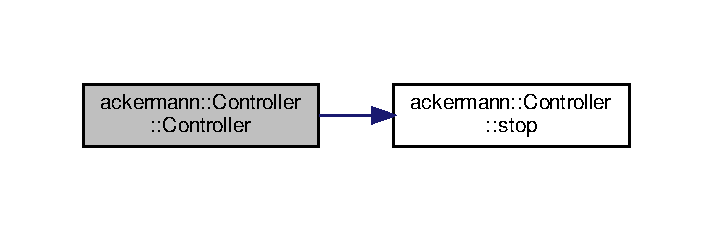
\includegraphics[width=342pt]{classackermann_1_1_controller_a4bf9f0657a103e0144ef14f9b8a7c96e_cgraph}
\end{center}
\end{figure}


\subsection{Member Function Documentation}
\mbox{\Hypertarget{classackermann_1_1_controller_a4af9cff4fa372a7bd245fe50aaf05859}\label{classackermann_1_1_controller_a4af9cff4fa372a7bd245fe50aaf05859}} 
\index{ackermann\+::\+Controller@{ackermann\+::\+Controller}!get\+Command@{get\+Command}}
\index{get\+Command@{get\+Command}!ackermann\+::\+Controller@{ackermann\+::\+Controller}}
\subsubsection{\texorpdfstring{get\+Command()}{getCommand()}}
{\footnotesize\ttfamily void ackermann\+::\+Controller\+::get\+Command (\begin{DoxyParamCaption}\item[{double \&}]{throttle,  }\item[{double \&}]{steering }\end{DoxyParamCaption}) const}



Get the current system command (speed, heading); return as parameters specified. 

This represents the main point of access for a polling architecture, i.\+e. an external control loop would periodically update the controller with the true system state and request command updates.


\begin{DoxyParams}{Parameters}
{\em throttle} & The latest throttle command (limited between \mbox{[}0,1\mbox{]}). \\
\hline
{\em steering} & The latest steering angle command (rad). \\
\hline
\end{DoxyParams}
\mbox{\Hypertarget{classackermann_1_1_controller_ad768d0fdc4ad85510ba90af05ef6e4c4}\label{classackermann_1_1_controller_ad768d0fdc4ad85510ba90af05ef6e4c4}} 
\index{ackermann\+::\+Controller@{ackermann\+::\+Controller}!get\+Goal@{get\+Goal}}
\index{get\+Goal@{get\+Goal}!ackermann\+::\+Controller@{ackermann\+::\+Controller}}
\subsubsection{\texorpdfstring{get\+Goal()}{getGoal()}}
{\footnotesize\ttfamily void ackermann\+::\+Controller\+::get\+Goal (\begin{DoxyParamCaption}\item[{double \&}]{speed,  }\item[{double \&}]{heading }\end{DoxyParamCaption}) const}



Get the current system setpoint (speed, heading); return as parameters specified. 


\begin{DoxyParams}{Parameters}
{\em heading} & The current vehicle heading setpoint (rad). \\
\hline
{\em speed} & The current vehicle speed setpoint (m/s). \\
\hline
\end{DoxyParams}
\mbox{\Hypertarget{classackermann_1_1_controller_a6a282c7083ce5a240d5e8e71782cb106}\label{classackermann_1_1_controller_a6a282c7083ce5a240d5e8e71782cb106}} 
\index{ackermann\+::\+Controller@{ackermann\+::\+Controller}!get\+State@{get\+State}}
\index{get\+State@{get\+State}!ackermann\+::\+Controller@{ackermann\+::\+Controller}}
\subsubsection{\texorpdfstring{get\+State()}{getState()}}
{\footnotesize\ttfamily void ackermann\+::\+Controller\+::get\+State (\begin{DoxyParamCaption}\item[{double \&}]{speed,  }\item[{double \&}]{heading }\end{DoxyParamCaption}) const}



Get the current state (speed, heading) of the system; return as parameters specified. 


\begin{DoxyParams}{Parameters}
{\em heading} & The estimated vehicle heading (rad). \\
\hline
{\em speed} & The estimated vehicle speed (m/s). \\
\hline
\end{DoxyParams}
\mbox{\Hypertarget{classackermann_1_1_controller_ab1831f2b1e80c29e5d110c55e11e2d2e}\label{classackermann_1_1_controller_ab1831f2b1e80c29e5d110c55e11e2d2e}} 
\index{ackermann\+::\+Controller@{ackermann\+::\+Controller}!get\+Wheel\+Lin\+Vel@{get\+Wheel\+Lin\+Vel}}
\index{get\+Wheel\+Lin\+Vel@{get\+Wheel\+Lin\+Vel}!ackermann\+::\+Controller@{ackermann\+::\+Controller}}
\subsubsection{\texorpdfstring{get\+Wheel\+Lin\+Vel()}{getWheelLinVel()}}
{\footnotesize\ttfamily void ackermann\+::\+Controller\+::get\+Wheel\+Lin\+Vel (\begin{DoxyParamCaption}\item[{double \&}]{left\+\_\+front,  }\item[{double \&}]{right\+\_\+front,  }\item[{double \&}]{left\+\_\+rear,  }\item[{double \&}]{right\+\_\+rear }\end{DoxyParamCaption}) const}



Get the current system wheel speeds; return as parameters specified. 


\begin{DoxyParams}{Parameters}
{\em left\+\_\+front} & The left front wheel velocity (m/s). \\
\hline
{\em right\+\_\+front} & The right front wheel velocity (m/s). \\
\hline
{\em left\+\_\+rear} & The left rear wheel velocity (m/s). \\
\hline
{\em right\+\_\+rear} & The right rear wheel velocity (m/s). \\
\hline
\end{DoxyParams}
\mbox{\Hypertarget{classackermann_1_1_controller_ac42d34ea838ccf8e9f83199b5753c08e}\label{classackermann_1_1_controller_ac42d34ea838ccf8e9f83199b5753c08e}} 
\index{ackermann\+::\+Controller@{ackermann\+::\+Controller}!is\+Running@{is\+Running}}
\index{is\+Running@{is\+Running}!ackermann\+::\+Controller@{ackermann\+::\+Controller}}
\subsubsection{\texorpdfstring{is\+Running()}{isRunning()}}
{\footnotesize\ttfamily bool ackermann\+::\+Controller\+::is\+Running (\begin{DoxyParamCaption}{ }\end{DoxyParamCaption}) const}



Return true if the core execution thread is running. This is a useful utility for testing. 

\begin{DoxyReturn}{Returns}
\+: Whether or not the core control loop is executing. 
\end{DoxyReturn}
\mbox{\Hypertarget{classackermann_1_1_controller_a2c048f93364371bb99445b68cb4ad064}\label{classackermann_1_1_controller_a2c048f93364371bb99445b68cb4ad064}} 
\index{ackermann\+::\+Controller@{ackermann\+::\+Controller}!set\+Goal@{set\+Goal}}
\index{set\+Goal@{set\+Goal}!ackermann\+::\+Controller@{ackermann\+::\+Controller}}
\subsubsection{\texorpdfstring{set\+Goal()}{setGoal()}}
{\footnotesize\ttfamily void ackermann\+::\+Controller\+::set\+Goal (\begin{DoxyParamCaption}\item[{const double}]{speed,  }\item[{const double}]{heading }\end{DoxyParamCaption})}



Set the current system setpoint (speed, heading). 

This sets a new target for our control loop. Expected usage is to call this method before calling \textquotesingle{}start\textquotesingle{}, although concurrent execution is supported.


\begin{DoxyParams}{Parameters}
{\em heading} & The desired vehicle heading (rad). \\
\hline
{\em speed} & The desired vehicle speed (m/s). \\
\hline
\end{DoxyParams}
\mbox{\Hypertarget{classackermann_1_1_controller_aee37f9adf9e8b2ec31499c8f7838531d}\label{classackermann_1_1_controller_aee37f9adf9e8b2ec31499c8f7838531d}} 
\index{ackermann\+::\+Controller@{ackermann\+::\+Controller}!set\+State@{set\+State}}
\index{set\+State@{set\+State}!ackermann\+::\+Controller@{ackermann\+::\+Controller}}
\subsubsection{\texorpdfstring{set\+State()}{setState()}}
{\footnotesize\ttfamily void ackermann\+::\+Controller\+::set\+State (\begin{DoxyParamCaption}\item[{const double}]{speed,  }\item[{const double}]{heading }\end{DoxyParamCaption})}



Set the current state (speed, heading) of the system. 

This represents an update from external sensors as to our true system state. If this is not called the controller will continue open loop.


\begin{DoxyParams}{Parameters}
{\em heading} & The actual vehicle heading (rad) \\
\hline
{\em speed} & The actual vehicle speed (m/s). \\
\hline
\end{DoxyParams}
\mbox{\Hypertarget{classackermann_1_1_controller_a285777e5abee8b5ec7eb683410215a04}\label{classackermann_1_1_controller_a285777e5abee8b5ec7eb683410215a04}} 
\index{ackermann\+::\+Controller@{ackermann\+::\+Controller}!stop@{stop}}
\index{stop@{stop}!ackermann\+::\+Controller@{ackermann\+::\+Controller}}
\subsubsection{\texorpdfstring{stop()}{stop()}}
{\footnotesize\ttfamily void ackermann\+::\+Controller\+::stop (\begin{DoxyParamCaption}\item[{bool}]{block = {\ttfamily false} }\end{DoxyParamCaption})}



Stop execution of a control loop and rejoin. This also calls \hyperlink{classackermann_1_1_controller_ab225ab7b942ed1590cc91b0343860924}{reset()} to clear any state variables. 

@ param block\+: Optionally wait for any running thread to rejoin. Default false. Here is the caller graph for this function\+:
\nopagebreak
\begin{figure}[H]
\begin{center}
\leavevmode
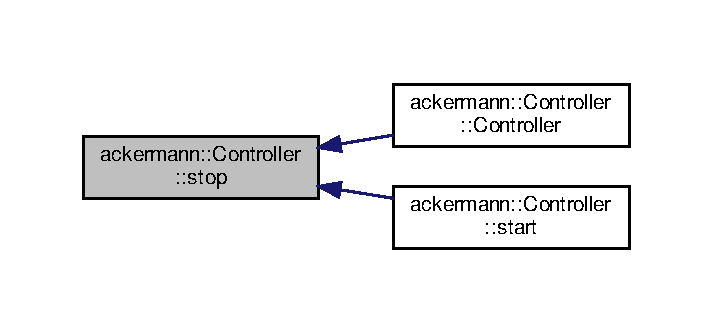
\includegraphics[width=342pt]{classackermann_1_1_controller_a285777e5abee8b5ec7eb683410215a04_icgraph}
\end{center}
\end{figure}


The documentation for this class was generated from the following files\+:\begin{DoxyCompactItemize}
\item 
include/\hyperlink{_controller_8hpp}{Controller.\+hpp}\item 
app/Controller.\+cpp\end{DoxyCompactItemize}

\hypertarget{classackermann_1_1_limits}{}\section{ackermann\+:\+:Limits Class Reference}
\label{classackermann_1_1_limits}\index{ackermann\+::\+Limits@{ackermann\+::\+Limits}}


Class used to apply known limits to a given desired control signal.  




{\ttfamily \#include $<$Limits.\+hpp$>$}

\subsection*{Public Member Functions}
\begin{DoxyCompactItemize}
\item 
\hyperlink{classackermann_1_1_limits_ab33a83c243c38ae9f046c77d49a6de58}{Limits} (const std\+::shared\+\_\+ptr$<$ const \hyperlink{structackermann_1_1_params}{Params} $>$ \&params)
\begin{DoxyCompactList}\small\item\em Constructor. \end{DoxyCompactList}\item 
void \hyperlink{classackermann_1_1_limits_a1fcf66ef8f8161d38e3d77c1e5acfb92}{limit} (const double current\+\_\+speed, const double current\+\_\+steering, const double current\+\_\+steering\+\_\+vel, double \&desired\+\_\+throttle, double \&desired\+\_\+steering, double \&desired\+\_\+steering\+\_\+vel, double dt) const
\begin{DoxyCompactList}\small\item\em Apply known limits to the given controller command. \end{DoxyCompactList}\item 
double \hyperlink{classackermann_1_1_limits_a0e75c61fc7d5d90c6f64af78d8cf76ff}{throttle\+To\+Speed} (double throttle) const
\begin{DoxyCompactList}\small\item\em Use Parameters structure to convert throttle to speed as a function of maximum allowable speed. \end{DoxyCompactList}\item 
double \hyperlink{classackermann_1_1_limits_abb347d9d57d22dfe47ef704ea6d10d7d}{speed\+To\+Throttle} (double speed) const
\begin{DoxyCompactList}\small\item\em Use Parameters structure to convert speed to throttle as a function of maximum allowable speed. \end{DoxyCompactList}\item 
double \hyperlink{classackermann_1_1_limits_a7fb25c558450b31945d1b13db4573a08}{shortest\+Arc\+To\+Turn} (double current\+\_\+heading, double desired\+\_\+heading) const
\begin{DoxyCompactList}\small\item\em Calculate the direction to minimize turning angle (eg, don\textquotesingle{}t turn 270deg right if you can turn 90deg left. \end{DoxyCompactList}\item 
double \hyperlink{classackermann_1_1_limits_a18e0ace6fde91bf5b641197dafbd5f57}{bound\+Heading} (const double heading) const
\begin{DoxyCompactList}\small\item\em Bound heading to \mbox{[}-\/pi,pi) range; prevents odd behavior. \end{DoxyCompactList}\end{DoxyCompactItemize}


\subsection{Detailed Description}
Class used to apply known limits to a given desired control signal. 

\subsection{Constructor \& Destructor Documentation}
\mbox{\Hypertarget{classackermann_1_1_limits_ab33a83c243c38ae9f046c77d49a6de58}\label{classackermann_1_1_limits_ab33a83c243c38ae9f046c77d49a6de58}} 
\index{ackermann\+::\+Limits@{ackermann\+::\+Limits}!Limits@{Limits}}
\index{Limits@{Limits}!ackermann\+::\+Limits@{ackermann\+::\+Limits}}
\subsubsection{\texorpdfstring{Limits()}{Limits()}}
{\footnotesize\ttfamily ackermann\+::\+Limits\+::\+Limits (\begin{DoxyParamCaption}\item[{const std\+::shared\+\_\+ptr$<$ const \hyperlink{structackermann_1_1_params}{Params} $>$ \&}]{params }\end{DoxyParamCaption})\hspace{0.3cm}{\ttfamily [explicit]}}



Constructor. 


\begin{DoxyParams}{Parameters}
{\em params} & Shared pointer detailing rover characteristic parameters \\
\hline
\end{DoxyParams}


\subsection{Member Function Documentation}
\mbox{\Hypertarget{classackermann_1_1_limits_a18e0ace6fde91bf5b641197dafbd5f57}\label{classackermann_1_1_limits_a18e0ace6fde91bf5b641197dafbd5f57}} 
\index{ackermann\+::\+Limits@{ackermann\+::\+Limits}!bound\+Heading@{bound\+Heading}}
\index{bound\+Heading@{bound\+Heading}!ackermann\+::\+Limits@{ackermann\+::\+Limits}}
\subsubsection{\texorpdfstring{bound\+Heading()}{boundHeading()}}
{\footnotesize\ttfamily double ackermann\+::\+Limits\+::bound\+Heading (\begin{DoxyParamCaption}\item[{const double}]{heading }\end{DoxyParamCaption}) const}



Bound heading to \mbox{[}-\/pi,pi) range; prevents odd behavior. 


\begin{DoxyParams}{Parameters}
{\em current\+\_\+heading} & Current heading in radians \\
\hline
{\em desired\+\_\+heading} & Desired heading in radians \\
\hline
\end{DoxyParams}
\begin{DoxyReturn}{Returns}
Bound heading in radians 
\end{DoxyReturn}
\mbox{\Hypertarget{classackermann_1_1_limits_a1fcf66ef8f8161d38e3d77c1e5acfb92}\label{classackermann_1_1_limits_a1fcf66ef8f8161d38e3d77c1e5acfb92}} 
\index{ackermann\+::\+Limits@{ackermann\+::\+Limits}!limit@{limit}}
\index{limit@{limit}!ackermann\+::\+Limits@{ackermann\+::\+Limits}}
\subsubsection{\texorpdfstring{limit()}{limit()}}
{\footnotesize\ttfamily void ackermann\+::\+Limits\+::limit (\begin{DoxyParamCaption}\item[{const double}]{current\+\_\+speed,  }\item[{const double}]{current\+\_\+steering,  }\item[{const double}]{current\+\_\+steering\+\_\+vel,  }\item[{double \&}]{desired\+\_\+throttle,  }\item[{double \&}]{desired\+\_\+steering,  }\item[{double \&}]{desired\+\_\+steering\+\_\+vel,  }\item[{double}]{dt }\end{DoxyParamCaption}) const}



Apply known limits to the given controller command. 

Apply known kinematic constraints (velocity, acceleration, angular velocity, angular acceleration) to the given potential commands, and return the limited version. (Return paramaters noted)


\begin{DoxyParams}{Parameters}
{\em current\+\_\+speed} & Current speed in (m/s). \\
\hline
{\em current\+\_\+steering} & Current commanded steering angle (rad). \\
\hline
{\em desired\+\_\+thottle} & (Return Parameter) Desired throttle (generally \mbox{[}0,1\mbox{]}). \\
\hline
{\em desired\+\_\+steering} & (Return Parameter) Desired steering angle (rad). \\
\hline
{\em desired\+\_\+steering\+\_\+vel} & (Return parameter) Desired steering velocity (rad/s). \\
\hline
{\em dt} & Fixed time step between commands (s). \\
\hline
\end{DoxyParams}
Here is the call graph for this function\+:
\nopagebreak
\begin{figure}[H]
\begin{center}
\leavevmode
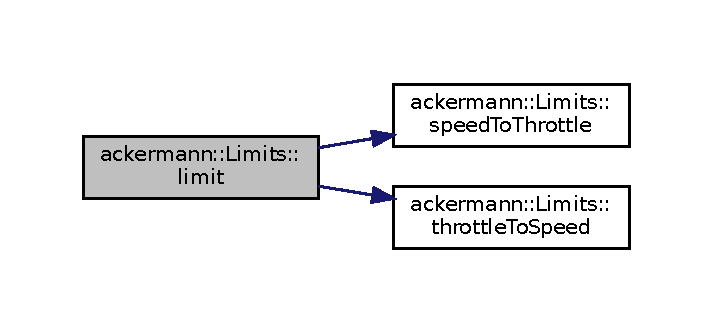
\includegraphics[width=322pt]{classackermann_1_1_limits_a1fcf66ef8f8161d38e3d77c1e5acfb92_cgraph}
\end{center}
\end{figure}
\mbox{\Hypertarget{classackermann_1_1_limits_a7fb25c558450b31945d1b13db4573a08}\label{classackermann_1_1_limits_a7fb25c558450b31945d1b13db4573a08}} 
\index{ackermann\+::\+Limits@{ackermann\+::\+Limits}!shortest\+Arc\+To\+Turn@{shortest\+Arc\+To\+Turn}}
\index{shortest\+Arc\+To\+Turn@{shortest\+Arc\+To\+Turn}!ackermann\+::\+Limits@{ackermann\+::\+Limits}}
\subsubsection{\texorpdfstring{shortest\+Arc\+To\+Turn()}{shortestArcToTurn()}}
{\footnotesize\ttfamily double ackermann\+::\+Limits\+::shortest\+Arc\+To\+Turn (\begin{DoxyParamCaption}\item[{double}]{current\+\_\+heading,  }\item[{double}]{desired\+\_\+heading }\end{DoxyParamCaption}) const}



Calculate the direction to minimize turning angle (eg, don\textquotesingle{}t turn 270deg right if you can turn 90deg left. 


\begin{DoxyParams}{Parameters}
{\em current\+\_\+heading} & Current heading in radians \\
\hline
{\em desired\+\_\+heading} & Desired heading in radians \\
\hline
\end{DoxyParams}
\begin{DoxyReturn}{Returns}
Angle and direction (+/-\/) to turn (rad) 
\end{DoxyReturn}
\mbox{\Hypertarget{classackermann_1_1_limits_abb347d9d57d22dfe47ef704ea6d10d7d}\label{classackermann_1_1_limits_abb347d9d57d22dfe47ef704ea6d10d7d}} 
\index{ackermann\+::\+Limits@{ackermann\+::\+Limits}!speed\+To\+Throttle@{speed\+To\+Throttle}}
\index{speed\+To\+Throttle@{speed\+To\+Throttle}!ackermann\+::\+Limits@{ackermann\+::\+Limits}}
\subsubsection{\texorpdfstring{speed\+To\+Throttle()}{speedToThrottle()}}
{\footnotesize\ttfamily double ackermann\+::\+Limits\+::speed\+To\+Throttle (\begin{DoxyParamCaption}\item[{double}]{speed }\end{DoxyParamCaption}) const}



Use Parameters structure to convert speed to throttle as a function of maximum allowable speed. 


\begin{DoxyParams}{Parameters}
{\em speed} & Speed in range of \mbox{[}0,max\+\_\+speed\mbox{]} \\
\hline
\end{DoxyParams}
\begin{DoxyReturn}{Returns}
Throttle position estimate from speed (linear relationship) \mbox{[}0,1\mbox{]} 
\end{DoxyReturn}
Here is the caller graph for this function\+:
\nopagebreak
\begin{figure}[H]
\begin{center}
\leavevmode
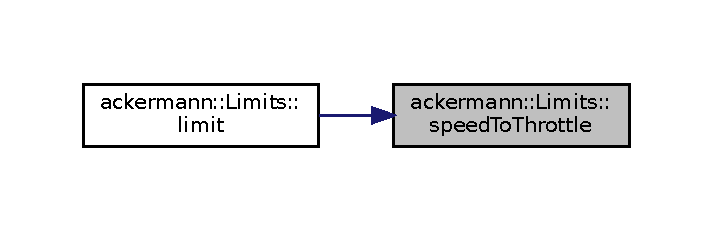
\includegraphics[width=322pt]{classackermann_1_1_limits_abb347d9d57d22dfe47ef704ea6d10d7d_icgraph}
\end{center}
\end{figure}
\mbox{\Hypertarget{classackermann_1_1_limits_a0e75c61fc7d5d90c6f64af78d8cf76ff}\label{classackermann_1_1_limits_a0e75c61fc7d5d90c6f64af78d8cf76ff}} 
\index{ackermann\+::\+Limits@{ackermann\+::\+Limits}!throttle\+To\+Speed@{throttle\+To\+Speed}}
\index{throttle\+To\+Speed@{throttle\+To\+Speed}!ackermann\+::\+Limits@{ackermann\+::\+Limits}}
\subsubsection{\texorpdfstring{throttle\+To\+Speed()}{throttleToSpeed()}}
{\footnotesize\ttfamily double ackermann\+::\+Limits\+::throttle\+To\+Speed (\begin{DoxyParamCaption}\item[{double}]{throttle }\end{DoxyParamCaption}) const}



Use Parameters structure to convert throttle to speed as a function of maximum allowable speed. 


\begin{DoxyParams}{Parameters}
{\em throttle} & Throttle setting in range of generally \mbox{[}0,1\mbox{]} \\
\hline
\end{DoxyParams}
\begin{DoxyReturn}{Returns}
Speed based on throttle input (linear relationship) (m/s) 
\end{DoxyReturn}
Here is the caller graph for this function\+:
\nopagebreak
\begin{figure}[H]
\begin{center}
\leavevmode
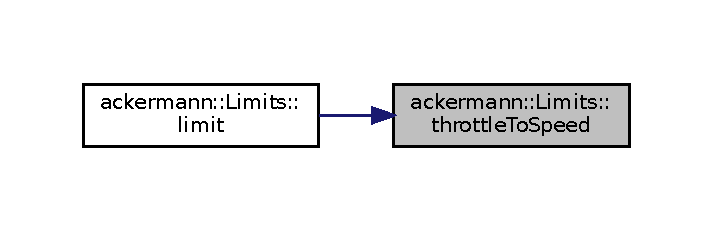
\includegraphics[width=322pt]{classackermann_1_1_limits_a0e75c61fc7d5d90c6f64af78d8cf76ff_icgraph}
\end{center}
\end{figure}


The documentation for this class was generated from the following files\+:\begin{DoxyCompactItemize}
\item 
include/\hyperlink{_limits_8hpp}{Limits.\+hpp}\item 
app/\hyperlink{_limits_8cpp}{Limits.\+cpp}\end{DoxyCompactItemize}

\hypertarget{classackermann_1_1_model}{}\doxysection{ackermann\+::Model Class Reference}
\label{classackermann_1_1_model}\index{ackermann::Model@{ackermann::Model}}


This class is used to further define a vehicle with Ackermann steering.  




{\ttfamily \#include $<$Model.\+hpp$>$}

\doxysubsection*{Public Member Functions}
\begin{DoxyCompactItemize}
\item 
\mbox{\hyperlink{classackermann_1_1_model_ad9fa277e47f993c8089a9c388880a32c}{Model}} (const std\+::shared\+\_\+ptr$<$ const \mbox{\hyperlink{structackermann_1_1_params}{Params}} $>$ \&params)
\begin{DoxyCompactList}\small\item\em Constructor. \end{DoxyCompactList}\item 
\mbox{\Hypertarget{classackermann_1_1_model_a6dc1b7ae5c40f0950b4944a63b192550}\label{classackermann_1_1_model_a6dc1b7ae5c40f0950b4944a63b192550}} 
void \mbox{\hyperlink{classackermann_1_1_model_a6dc1b7ae5c40f0950b4944a63b192550}{reset}} ()
\begin{DoxyCompactList}\small\item\em Reset system state variables to defaults. \end{DoxyCompactList}\item 
void \mbox{\hyperlink{classackermann_1_1_model_a109accf55eac34a33c9a5b2b8107e670}{set\+State}} (const double speed, const double heading)
\begin{DoxyCompactList}\small\item\em Set the current system state. \end{DoxyCompactList}\item 
void \mbox{\hyperlink{classackermann_1_1_model_a770662c33060369f437a098c944ca262}{get\+State}} (double \&speed, double \&heading) const
\begin{DoxyCompactList}\small\item\em Get the current state estimate; return as parameters specified. \end{DoxyCompactList}\item 
void \mbox{\hyperlink{classackermann_1_1_model_a09d9ac604f91d339eae4b18a85db9732}{set\+Goal}} (const double speed, const double heading)
\begin{DoxyCompactList}\small\item\em Set the target setpoint. \end{DoxyCompactList}\item 
void \mbox{\hyperlink{classackermann_1_1_model_a37c42fe7705a2b3106b0faff813bfcad}{get\+Goal}} (double \&speed, double \&heading) const
\begin{DoxyCompactList}\small\item\em Get the current setpoint; return as parameters specified. \end{DoxyCompactList}\item 
void \mbox{\hyperlink{classackermann_1_1_model_a24f1fd6f59b6daa78b1f99f5f2029b56}{get\+Command}} (double \&throttle, double \&steering) const
\begin{DoxyCompactList}\small\item\em Get the current commanded throttle and steering angle; return as parameters specified. \end{DoxyCompactList}\item 
void \mbox{\hyperlink{classackermann_1_1_model_a3f0eaa6a1b63479e4d59689bc6e60c71}{get\+Command}} (double \&throttle, double \&steering, double \&steer\+\_\+vel) const
\begin{DoxyCompactList}\small\item\em Get the current commanded throttle and steering angle; return as parameters specified. \end{DoxyCompactList}\item 
void \mbox{\hyperlink{classackermann_1_1_model_a62226204f92b8c1c7cca0a11f616d7fd}{command}} (double desired\+\_\+speed, double steering, const double dt)
\begin{DoxyCompactList}\small\item\em Simulate execution of the given throttle and steering commands. \end{DoxyCompactList}\item 
void \mbox{\hyperlink{classackermann_1_1_model_a4b91f4da42041ac667e49116b4f1040d}{get\+Error}} (double \&speed\+\_\+error, double \&heading\+\_\+error) const
\begin{DoxyCompactList}\small\item\em Return the current error between desired and setpoint; return as parameters specified. \end{DoxyCompactList}\item 
void \mbox{\hyperlink{classackermann_1_1_model_a571711ea578e1ccaa7bc23528a53ba95}{get\+Wheel\+Lin\+Vel}} (double \&wheel\+\_\+\+Left\+Front, double \&wheel\+\_\+\+Right\+Front, double \&wheel\+\_\+\+Left\+Rear, double \&wheel\+\_\+\+Right\+Rear) const
\begin{DoxyCompactList}\small\item\em Return the current linear velocity at each wheel; used for calculating wheel speed with tire information. Return as parameters specified. \end{DoxyCompactList}\end{DoxyCompactItemize}


\doxysubsection{Detailed Description}
This class is used to further define a vehicle with Ackermann steering. 

\doxysubsection{Constructor \& Destructor Documentation}
\mbox{\Hypertarget{classackermann_1_1_model_ad9fa277e47f993c8089a9c388880a32c}\label{classackermann_1_1_model_ad9fa277e47f993c8089a9c388880a32c}} 
\index{ackermann::Model@{ackermann::Model}!Model@{Model}}
\index{Model@{Model}!ackermann::Model@{ackermann::Model}}
\doxysubsubsection{\texorpdfstring{Model()}{Model()}}
{\footnotesize\ttfamily ackermann\+::\+Model\+::\+Model (\begin{DoxyParamCaption}\item[{const std\+::shared\+\_\+ptr$<$ const \mbox{\hyperlink{structackermann_1_1_params}{Params}} $>$ \&}]{params }\end{DoxyParamCaption})\hspace{0.3cm}{\ttfamily [explicit]}}



Constructor. 


\begin{DoxyParams}{Parameters}
{\em params} & Shared pointer detailing rover characteristic parameters \\
\hline
\end{DoxyParams}
Here is the call graph for this function\+:
\nopagebreak
\begin{figure}[H]
\begin{center}
\leavevmode
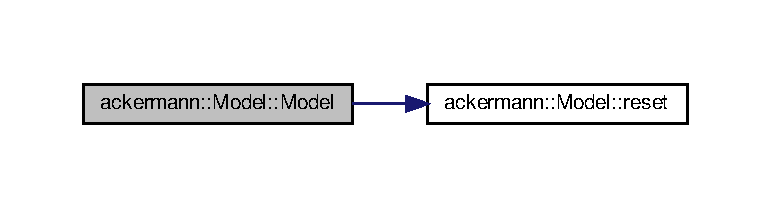
\includegraphics[width=350pt]{classackermann_1_1_model_ad9fa277e47f993c8089a9c388880a32c_cgraph}
\end{center}
\end{figure}


\doxysubsection{Member Function Documentation}
\mbox{\Hypertarget{classackermann_1_1_model_a62226204f92b8c1c7cca0a11f616d7fd}\label{classackermann_1_1_model_a62226204f92b8c1c7cca0a11f616d7fd}} 
\index{ackermann::Model@{ackermann::Model}!command@{command}}
\index{command@{command}!ackermann::Model@{ackermann::Model}}
\doxysubsubsection{\texorpdfstring{command()}{command()}}
{\footnotesize\ttfamily void ackermann\+::\+Model\+::command (\begin{DoxyParamCaption}\item[{double}]{desired\+\_\+speed,  }\item[{double}]{steering,  }\item[{const double}]{dt }\end{DoxyParamCaption})}



Simulate execution of the given throttle and steering commands. 


\begin{DoxyParams}{Parameters}
{\em throttle} & The commanded throttle (\mbox{[}0,1\mbox{]}). \\
\hline
{\em steering} & The commanded steering angle (rad). \\
\hline
{\em dt} & The amount of time to simulate over (s). \\
\hline
\end{DoxyParams}
\mbox{\Hypertarget{classackermann_1_1_model_a24f1fd6f59b6daa78b1f99f5f2029b56}\label{classackermann_1_1_model_a24f1fd6f59b6daa78b1f99f5f2029b56}} 
\index{ackermann::Model@{ackermann::Model}!getCommand@{getCommand}}
\index{getCommand@{getCommand}!ackermann::Model@{ackermann::Model}}
\doxysubsubsection{\texorpdfstring{getCommand()}{getCommand()}\hspace{0.1cm}{\footnotesize\ttfamily [1/2]}}
{\footnotesize\ttfamily void ackermann\+::\+Model\+::get\+Command (\begin{DoxyParamCaption}\item[{double \&}]{throttle,  }\item[{double \&}]{steering }\end{DoxyParamCaption}) const}



Get the current commanded throttle and steering angle; return as parameters specified. 


\begin{DoxyParams}{Parameters}
{\em throttle} & The last commanded throttle (limited to \mbox{[}0,1\mbox{]}). \\
\hline
{\em steering} & The last commanded steering angle (rad). \\
\hline
\end{DoxyParams}
\mbox{\Hypertarget{classackermann_1_1_model_a3f0eaa6a1b63479e4d59689bc6e60c71}\label{classackermann_1_1_model_a3f0eaa6a1b63479e4d59689bc6e60c71}} 
\index{ackermann::Model@{ackermann::Model}!getCommand@{getCommand}}
\index{getCommand@{getCommand}!ackermann::Model@{ackermann::Model}}
\doxysubsubsection{\texorpdfstring{getCommand()}{getCommand()}\hspace{0.1cm}{\footnotesize\ttfamily [2/2]}}
{\footnotesize\ttfamily void ackermann\+::\+Model\+::get\+Command (\begin{DoxyParamCaption}\item[{double \&}]{throttle,  }\item[{double \&}]{steering,  }\item[{double \&}]{steer\+\_\+vel }\end{DoxyParamCaption}) const}



Get the current commanded throttle and steering angle; return as parameters specified. 


\begin{DoxyParams}{Parameters}
{\em throttle} & The last commanded throttle (limited to \mbox{[}0,1\mbox{]}). \\
\hline
{\em steering} & The last commanded steering angle (rad). \\
\hline
{\em steer\+\_\+vel} & The current steering angle velocity (rad/s). \\
\hline
\end{DoxyParams}
\mbox{\Hypertarget{classackermann_1_1_model_a4b91f4da42041ac667e49116b4f1040d}\label{classackermann_1_1_model_a4b91f4da42041ac667e49116b4f1040d}} 
\index{ackermann::Model@{ackermann::Model}!getError@{getError}}
\index{getError@{getError}!ackermann::Model@{ackermann::Model}}
\doxysubsubsection{\texorpdfstring{getError()}{getError()}}
{\footnotesize\ttfamily void ackermann\+::\+Model\+::get\+Error (\begin{DoxyParamCaption}\item[{double \&}]{speed\+\_\+error,  }\item[{double \&}]{heading\+\_\+error }\end{DoxyParamCaption}) const}



Return the current error between desired and setpoint; return as parameters specified. 


\begin{DoxyParams}{Parameters}
{\em speed\+\_\+error} & Current speed error (m/s). \\
\hline
{\em heading\+\_\+error} & Current heading error (rad). \\
\hline
\end{DoxyParams}
\mbox{\Hypertarget{classackermann_1_1_model_a37c42fe7705a2b3106b0faff813bfcad}\label{classackermann_1_1_model_a37c42fe7705a2b3106b0faff813bfcad}} 
\index{ackermann::Model@{ackermann::Model}!getGoal@{getGoal}}
\index{getGoal@{getGoal}!ackermann::Model@{ackermann::Model}}
\doxysubsubsection{\texorpdfstring{getGoal()}{getGoal()}}
{\footnotesize\ttfamily void ackermann\+::\+Model\+::get\+Goal (\begin{DoxyParamCaption}\item[{double \&}]{speed,  }\item[{double \&}]{heading }\end{DoxyParamCaption}) const}



Get the current setpoint; return as parameters specified. 


\begin{DoxyParams}{Parameters}
{\em speed} & Desired system speed (m/s). \\
\hline
{\em heading} & Desired system heading (rad). \\
\hline
\end{DoxyParams}
\mbox{\Hypertarget{classackermann_1_1_model_a770662c33060369f437a098c944ca262}\label{classackermann_1_1_model_a770662c33060369f437a098c944ca262}} 
\index{ackermann::Model@{ackermann::Model}!getState@{getState}}
\index{getState@{getState}!ackermann::Model@{ackermann::Model}}
\doxysubsubsection{\texorpdfstring{getState()}{getState()}}
{\footnotesize\ttfamily void ackermann\+::\+Model\+::get\+State (\begin{DoxyParamCaption}\item[{double \&}]{speed,  }\item[{double \&}]{heading }\end{DoxyParamCaption}) const}



Get the current state estimate; return as parameters specified. 


\begin{DoxyParams}{Parameters}
{\em speed} & Estimated system speed (m/s). \\
\hline
{\em heading} & Estimated system heading (rad). \\
\hline
\end{DoxyParams}
\mbox{\Hypertarget{classackermann_1_1_model_a571711ea578e1ccaa7bc23528a53ba95}\label{classackermann_1_1_model_a571711ea578e1ccaa7bc23528a53ba95}} 
\index{ackermann::Model@{ackermann::Model}!getWheelLinVel@{getWheelLinVel}}
\index{getWheelLinVel@{getWheelLinVel}!ackermann::Model@{ackermann::Model}}
\doxysubsubsection{\texorpdfstring{getWheelLinVel()}{getWheelLinVel()}}
{\footnotesize\ttfamily void ackermann\+::\+Model\+::get\+Wheel\+Lin\+Vel (\begin{DoxyParamCaption}\item[{double \&}]{wheel\+\_\+\+Left\+Front,  }\item[{double \&}]{wheel\+\_\+\+Right\+Front,  }\item[{double \&}]{wheel\+\_\+\+Left\+Rear,  }\item[{double \&}]{wheel\+\_\+\+Right\+Rear }\end{DoxyParamCaption}) const}



Return the current linear velocity at each wheel; used for calculating wheel speed with tire information. Return as parameters specified. 


\begin{DoxyParams}{Parameters}
{\em wheel\+\_\+\+Left\+Front\&} & Left front wheel linear velocity \\
\hline
{\em wheel\+\_\+\+Right\+Front\&} & Right front wheel linear velocity \\
\hline
{\em wheel\+\_\+\+Left\+Rear\&} & Left rear wheel linear velocity \\
\hline
{\em wheel\+\_\+\+Right\+Rear\&} & Right rear wheel linear velocity \\
\hline
\end{DoxyParams}
\mbox{\Hypertarget{classackermann_1_1_model_a09d9ac604f91d339eae4b18a85db9732}\label{classackermann_1_1_model_a09d9ac604f91d339eae4b18a85db9732}} 
\index{ackermann::Model@{ackermann::Model}!setGoal@{setGoal}}
\index{setGoal@{setGoal}!ackermann::Model@{ackermann::Model}}
\doxysubsubsection{\texorpdfstring{setGoal()}{setGoal()}}
{\footnotesize\ttfamily void ackermann\+::\+Model\+::set\+Goal (\begin{DoxyParamCaption}\item[{const double}]{speed,  }\item[{const double}]{heading }\end{DoxyParamCaption})}



Set the target setpoint. 


\begin{DoxyParams}{Parameters}
{\em speed} & Desired system speed (m/s). \\
\hline
{\em heading} & Desired system heading (rad). \\
\hline
\end{DoxyParams}
\mbox{\Hypertarget{classackermann_1_1_model_a109accf55eac34a33c9a5b2b8107e670}\label{classackermann_1_1_model_a109accf55eac34a33c9a5b2b8107e670}} 
\index{ackermann::Model@{ackermann::Model}!setState@{setState}}
\index{setState@{setState}!ackermann::Model@{ackermann::Model}}
\doxysubsubsection{\texorpdfstring{setState()}{setState()}}
{\footnotesize\ttfamily void ackermann\+::\+Model\+::set\+State (\begin{DoxyParamCaption}\item[{const double}]{speed,  }\item[{const double}]{heading }\end{DoxyParamCaption})}



Set the current system state. 


\begin{DoxyParams}{Parameters}
{\em speed} & Actual system speed (m/s) \\
\hline
{\em heading} & Actual system heading (rad). \\
\hline
\end{DoxyParams}


The documentation for this class was generated from the following files\+:\begin{DoxyCompactItemize}
\item 
include/\mbox{\hyperlink{_model_8hpp}{Model.\+hpp}}\item 
app/Model.\+cpp\end{DoxyCompactItemize}

\hypertarget{structackermann_1_1_params}{}\doxysection{ackermann\+::Params Struct Reference}
\label{structackermann_1_1_params}\index{ackermann::Params@{ackermann::Params}}


Structure containing rover characteristics and limitations.  




{\ttfamily \#include $<$Params.\+hpp$>$}

\doxysubsection*{Public Member Functions}
\begin{DoxyCompactItemize}
\item 
\mbox{\Hypertarget{structackermann_1_1_params_a4d036653d2b7f9e6cbfaea12d5dca6f4}\label{structackermann_1_1_params_a4d036653d2b7f9e6cbfaea12d5dca6f4}} 
{\bfseries Params} (double wheel\+\_\+base\+\_\+, double track\+\_\+width\+\_\+, double max\+\_\+steering\+\_\+angle\+\_\+, double kp\+\_\+speed\+\_\+, double kp\+\_\+heading\+\_\+)
\end{DoxyCompactItemize}
\doxysubsection*{Public Attributes}
\begin{DoxyCompactItemize}
\item 
\mbox{\Hypertarget{structackermann_1_1_params_a065f737848871356232ff7092baed140}\label{structackermann_1_1_params_a065f737848871356232ff7092baed140}} 
std\+::atomic$<$ double $>$ \mbox{\hyperlink{structackermann_1_1_params_a065f737848871356232ff7092baed140}{control\+\_\+frequency}} \{100.\+0\}
\begin{DoxyCompactList}\small\item\em Desired frequency of controller loop. \end{DoxyCompactList}\item 
\mbox{\Hypertarget{structackermann_1_1_params_ab41d61361183158ea37d6c8577dcad82}\label{structackermann_1_1_params_ab41d61361183158ea37d6c8577dcad82}} 
std\+::atomic$<$ double $>$ \mbox{\hyperlink{structackermann_1_1_params_ab41d61361183158ea37d6c8577dcad82}{velocity\+\_\+max}} \{10.\+0\}
\begin{DoxyCompactList}\small\item\em Maximum allowable velocity of rover (m/s). Used with throttle command for speed calculation. \end{DoxyCompactList}\item 
\mbox{\Hypertarget{structackermann_1_1_params_ad6c5babc5a52cf56d57ea664ca5a0c04}\label{structackermann_1_1_params_ad6c5babc5a52cf56d57ea664ca5a0c04}} 
std\+::atomic$<$ double $>$ \mbox{\hyperlink{structackermann_1_1_params_ad6c5babc5a52cf56d57ea664ca5a0c04}{velocity\+\_\+min}} \{0.\+0\}
\begin{DoxyCompactList}\small\item\em Minimum allowable velocity of rover (m/s). Backwards driving not yet implemented, set to 0 m/s until implemented.. \end{DoxyCompactList}\item 
\mbox{\Hypertarget{structackermann_1_1_params_a7273215906e350eb609b463398acbfba}\label{structackermann_1_1_params_a7273215906e350eb609b463398acbfba}} 
std\+::atomic$<$ double $>$ \mbox{\hyperlink{structackermann_1_1_params_a7273215906e350eb609b463398acbfba}{acceleration\+\_\+max}} \{50.\+0\}
\begin{DoxyCompactList}\small\item\em Maximum allowable acceleration of rover (m/s$^\wedge$2) \end{DoxyCompactList}\item 
\mbox{\Hypertarget{structackermann_1_1_params_a9b8d3b799a556afb69f3f8acd0abfa66}\label{structackermann_1_1_params_a9b8d3b799a556afb69f3f8acd0abfa66}} 
std\+::atomic$<$ double $>$ \mbox{\hyperlink{structackermann_1_1_params_a9b8d3b799a556afb69f3f8acd0abfa66}{acceleration\+\_\+min}} \{-\/50.\+0\}
\begin{DoxyCompactList}\small\item\em Minimum allowable acceleration of rover (e.\+g., braking) (m/s$^\wedge$2) \end{DoxyCompactList}\item 
std\+::atomic$<$ double $>$ \mbox{\hyperlink{structackermann_1_1_params_aad93f5ef58bf87db04c9e21f3c1067ca}{angular\+\_\+velocity\+\_\+max}}
\begin{DoxyCompactList}\small\item\em Maximum allowable (rightward) angular velocity of steering change (rad/s) \end{DoxyCompactList}\item 
std\+::atomic$<$ double $>$ \mbox{\hyperlink{structackermann_1_1_params_a20071280825a5dfdf0eba12fa45c6886}{angular\+\_\+velocity\+\_\+min}}
\begin{DoxyCompactList}\small\item\em Minimum allowable (leftward) angular velocity of steering change (rad/s) \end{DoxyCompactList}\item 
std\+::atomic$<$ double $>$ \mbox{\hyperlink{structackermann_1_1_params_a69fd058a9c869f1db12b030a99f3141d}{angular\+\_\+acceleration\+\_\+max}}
\begin{DoxyCompactList}\small\item\em Maximum allowable (rightward) angular acceleration of steering change (rad/s$^\wedge$2) \end{DoxyCompactList}\item 
std\+::atomic$<$ double $>$ \mbox{\hyperlink{structackermann_1_1_params_a5baf993ebf740d79eeb1e19e041ceb8e}{angular\+\_\+acceleration\+\_\+min}}
\begin{DoxyCompactList}\small\item\em Minimum allowable (leftward) angular acceleration of steering change (rad/s$^\wedge$2) \end{DoxyCompactList}\item 
\mbox{\Hypertarget{structackermann_1_1_params_a77e9e8355199625173a243b96963a543}\label{structackermann_1_1_params_a77e9e8355199625173a243b96963a543}} 
std\+::atomic$<$ double $>$ \mbox{\hyperlink{structackermann_1_1_params_a77e9e8355199625173a243b96963a543}{throttle\+\_\+max}} \{1.\+0\}
\begin{DoxyCompactList}\small\item\em Maximum throttle setting -\/ should set to 1.\+0. \end{DoxyCompactList}\item 
\mbox{\Hypertarget{structackermann_1_1_params_a105dda9186730914c63f6e39593d0e77}\label{structackermann_1_1_params_a105dda9186730914c63f6e39593d0e77}} 
std\+::atomic$<$ double $>$ \mbox{\hyperlink{structackermann_1_1_params_a105dda9186730914c63f6e39593d0e77}{throttle\+\_\+min}} \{0.\+0\}
\begin{DoxyCompactList}\small\item\em Minimum throttle setting -\/ should set to 0.\+0. \end{DoxyCompactList}\item 
\mbox{\Hypertarget{structackermann_1_1_params_adcbcf331c428efc01e2be5da332b6e99}\label{structackermann_1_1_params_adcbcf331c428efc01e2be5da332b6e99}} 
const std\+::shared\+\_\+ptr$<$ \mbox{\hyperlink{structackermann_1_1_p_i_d_params}{P\+I\+D\+Params}} $>$ \mbox{\hyperlink{structackermann_1_1_params_adcbcf331c428efc01e2be5da332b6e99}{pid\+\_\+speed}}
\begin{DoxyCompactList}\small\item\em Speed controller \mbox{\hyperlink{classackermann_1_1_p_i_d}{P\+ID}} parameters. \end{DoxyCompactList}\item 
\mbox{\Hypertarget{structackermann_1_1_params_ab8ef5ea67822f187c7a03f94e20a24d0}\label{structackermann_1_1_params_ab8ef5ea67822f187c7a03f94e20a24d0}} 
const std\+::shared\+\_\+ptr$<$ \mbox{\hyperlink{structackermann_1_1_p_i_d_params}{P\+I\+D\+Params}} $>$ \mbox{\hyperlink{structackermann_1_1_params_ab8ef5ea67822f187c7a03f94e20a24d0}{pid\+\_\+heading}}
\begin{DoxyCompactList}\small\item\em Heading controller \mbox{\hyperlink{classackermann_1_1_p_i_d}{P\+ID}} parameters. \end{DoxyCompactList}\item 
\mbox{\Hypertarget{structackermann_1_1_params_a68ecfa01510e295926dd23b1cfb1d83a}\label{structackermann_1_1_params_a68ecfa01510e295926dd23b1cfb1d83a}} 
std\+::atomic$<$ double $>$ \mbox{\hyperlink{structackermann_1_1_params_a68ecfa01510e295926dd23b1cfb1d83a}{wheel\+\_\+base}}
\begin{DoxyCompactList}\small\item\em Length between front and rear axles (m) \end{DoxyCompactList}\item 
\mbox{\Hypertarget{structackermann_1_1_params_a429093b21328bce330f930f55c1e3b3c}\label{structackermann_1_1_params_a429093b21328bce330f930f55c1e3b3c}} 
std\+::atomic$<$ double $>$ \mbox{\hyperlink{structackermann_1_1_params_a429093b21328bce330f930f55c1e3b3c}{track\+\_\+width}}
\begin{DoxyCompactList}\small\item\em Width between left and right tires (m) \end{DoxyCompactList}\item 
\mbox{\Hypertarget{structackermann_1_1_params_a7bfb774e679c8e5372ec512a62f5d0ce}\label{structackermann_1_1_params_a7bfb774e679c8e5372ec512a62f5d0ce}} 
std\+::atomic$<$ double $>$ \mbox{\hyperlink{structackermann_1_1_params_a7bfb774e679c8e5372ec512a62f5d0ce}{max\+\_\+steering\+\_\+angle}}
\begin{DoxyCompactList}\small\item\em Maximum angle of steering mechanism (rad) \end{DoxyCompactList}\end{DoxyCompactItemize}


\doxysubsection{Detailed Description}
Structure containing rover characteristics and limitations. 

\doxysubsection{Member Data Documentation}
\mbox{\Hypertarget{structackermann_1_1_params_a69fd058a9c869f1db12b030a99f3141d}\label{structackermann_1_1_params_a69fd058a9c869f1db12b030a99f3141d}} 
\index{ackermann::Params@{ackermann::Params}!angular\_acceleration\_max@{angular\_acceleration\_max}}
\index{angular\_acceleration\_max@{angular\_acceleration\_max}!ackermann::Params@{ackermann::Params}}
\doxysubsubsection{\texorpdfstring{angular\_acceleration\_max}{angular\_acceleration\_max}}
{\footnotesize\ttfamily std\+::atomic$<$double$>$ ackermann\+::\+Params\+::angular\+\_\+acceleration\+\_\+max}

{\bfseries Initial value\+:}
\begin{DoxyCode}{0}
\DoxyCodeLine{\{}
\DoxyCodeLine{    std::numeric\_limits<double>::max()\}}

\end{DoxyCode}


Maximum allowable (rightward) angular acceleration of steering change (rad/s$^\wedge$2) 

\mbox{\Hypertarget{structackermann_1_1_params_a5baf993ebf740d79eeb1e19e041ceb8e}\label{structackermann_1_1_params_a5baf993ebf740d79eeb1e19e041ceb8e}} 
\index{ackermann::Params@{ackermann::Params}!angular\_acceleration\_min@{angular\_acceleration\_min}}
\index{angular\_acceleration\_min@{angular\_acceleration\_min}!ackermann::Params@{ackermann::Params}}
\doxysubsubsection{\texorpdfstring{angular\_acceleration\_min}{angular\_acceleration\_min}}
{\footnotesize\ttfamily std\+::atomic$<$double$>$ ackermann\+::\+Params\+::angular\+\_\+acceleration\+\_\+min}

{\bfseries Initial value\+:}
\begin{DoxyCode}{0}
\DoxyCodeLine{\{}
\DoxyCodeLine{    std::numeric\_limits<double>::lowest()\}}

\end{DoxyCode}


Minimum allowable (leftward) angular acceleration of steering change (rad/s$^\wedge$2) 

\mbox{\Hypertarget{structackermann_1_1_params_aad93f5ef58bf87db04c9e21f3c1067ca}\label{structackermann_1_1_params_aad93f5ef58bf87db04c9e21f3c1067ca}} 
\index{ackermann::Params@{ackermann::Params}!angular\_velocity\_max@{angular\_velocity\_max}}
\index{angular\_velocity\_max@{angular\_velocity\_max}!ackermann::Params@{ackermann::Params}}
\doxysubsubsection{\texorpdfstring{angular\_velocity\_max}{angular\_velocity\_max}}
{\footnotesize\ttfamily std\+::atomic$<$double$>$ ackermann\+::\+Params\+::angular\+\_\+velocity\+\_\+max}

{\bfseries Initial value\+:}
\begin{DoxyCode}{0}
\DoxyCodeLine{\{}
\DoxyCodeLine{    std::numeric\_limits<double>::max()\}}

\end{DoxyCode}


Maximum allowable (rightward) angular velocity of steering change (rad/s) 

\mbox{\Hypertarget{structackermann_1_1_params_a20071280825a5dfdf0eba12fa45c6886}\label{structackermann_1_1_params_a20071280825a5dfdf0eba12fa45c6886}} 
\index{ackermann::Params@{ackermann::Params}!angular\_velocity\_min@{angular\_velocity\_min}}
\index{angular\_velocity\_min@{angular\_velocity\_min}!ackermann::Params@{ackermann::Params}}
\doxysubsubsection{\texorpdfstring{angular\_velocity\_min}{angular\_velocity\_min}}
{\footnotesize\ttfamily std\+::atomic$<$double$>$ ackermann\+::\+Params\+::angular\+\_\+velocity\+\_\+min}

{\bfseries Initial value\+:}
\begin{DoxyCode}{0}
\DoxyCodeLine{\{}
\DoxyCodeLine{    std::numeric\_limits<double>::lowest()\}}

\end{DoxyCode}


Minimum allowable (leftward) angular velocity of steering change (rad/s) 



The documentation for this struct was generated from the following file\+:\begin{DoxyCompactItemize}
\item 
include/\mbox{\hyperlink{_params_8hpp}{Params.\+hpp}}\end{DoxyCompactItemize}

\hypertarget{classackermann_1_1_p_i_d}{}\section{ackermann\+:\+:P\+ID Class Reference}
\label{classackermann_1_1_p_i_d}\index{ackermann\+::\+P\+ID@{ackermann\+::\+P\+ID}}


This class implements a \hyperlink{classackermann_1_1_p_i_d}{P\+ID} controller with max/min clamping of output values to prevent integral windup.  




{\ttfamily \#include $<$P\+I\+D.\+hpp$>$}

\subsection*{Public Member Functions}
\begin{DoxyCompactItemize}
\item 
\hyperlink{classackermann_1_1_p_i_d_a98e96878fcc3373f22d783b78c7cf0d9}{P\+ID} (const std\+::shared\+\_\+ptr$<$ const \hyperlink{structackermann_1_1_p_i_d_params}{P\+I\+D\+Params} $>$ \&params, double out\+\_\+min\+Limit=std\+::numeric\+\_\+limits$<$ double $>$\+::lowest(), double out\+\_\+max\+Limit=std\+::numeric\+\_\+limits$<$ double $>$\+::max())
\begin{DoxyCompactList}\small\item\em Constructor. \end{DoxyCompactList}\item 
double \hyperlink{classackermann_1_1_p_i_d_a3257bf60c93eb2a3b18b48a40a480b2d}{get\+\_\+k\+\_\+p} () const
\begin{DoxyCompactList}\small\item\em Get the kP Proportional Gain. \end{DoxyCompactList}\item 
double \hyperlink{classackermann_1_1_p_i_d_a9845f8af09db7e901d319c53e4e43268}{get\+\_\+k\+\_\+i} () const
\begin{DoxyCompactList}\small\item\em Get the kI Integral Gain. \end{DoxyCompactList}\item 
double \hyperlink{classackermann_1_1_p_i_d_aaf565af4f72abcf148b8abe8880df6c3}{get\+\_\+k\+\_\+d} () const
\begin{DoxyCompactList}\small\item\em Get the kD Derivative Gain. \end{DoxyCompactList}\item 
double \hyperlink{classackermann_1_1_p_i_d_a6286415d935d49dceba543deb4356b42}{get\+Command} (double current\+\_\+error, double dt)
\begin{DoxyCompactList}\small\item\em Perform \hyperlink{classackermann_1_1_p_i_d}{P\+ID} Calculation. \end{DoxyCompactList}\item 
void \hyperlink{classackermann_1_1_p_i_d_a1f2e47eb9958ec5d1887bf7c5f82175a}{reset\+\_\+\+P\+ID} ()
\begin{DoxyCompactList}\small\item\em Reset the \hyperlink{classackermann_1_1_p_i_d}{P\+ID}. \end{DoxyCompactList}\end{DoxyCompactItemize}


\subsection{Detailed Description}
This class implements a \hyperlink{classackermann_1_1_p_i_d}{P\+ID} controller with max/min clamping of output values to prevent integral windup. 

\subsection{Constructor \& Destructor Documentation}
\mbox{\Hypertarget{classackermann_1_1_p_i_d_a98e96878fcc3373f22d783b78c7cf0d9}\label{classackermann_1_1_p_i_d_a98e96878fcc3373f22d783b78c7cf0d9}} 
\index{ackermann\+::\+P\+ID@{ackermann\+::\+P\+ID}!P\+ID@{P\+ID}}
\index{P\+ID@{P\+ID}!ackermann\+::\+P\+ID@{ackermann\+::\+P\+ID}}
\subsubsection{\texorpdfstring{P\+I\+D()}{PID()}}
{\footnotesize\ttfamily ackermann\+::\+P\+I\+D\+::\+P\+ID (\begin{DoxyParamCaption}\item[{const std\+::shared\+\_\+ptr$<$ const \hyperlink{structackermann_1_1_p_i_d_params}{P\+I\+D\+Params} $>$ \&}]{params,  }\item[{double}]{out\+\_\+min\+Limit = {\ttfamily std\+:\+:numeric\+\_\+limits$<$double$>$\+:\+:lowest()},  }\item[{double}]{out\+\_\+max\+Limit = {\ttfamily std\+:\+:numeric\+\_\+limits$<$double$>$\+:\+:max()} }\end{DoxyParamCaption})\hspace{0.3cm}{\ttfamily [explicit]}}



Constructor. 


\begin{DoxyParams}{Parameters}
{\em params} & Shared \hyperlink{structackermann_1_1_p_i_d_params}{P\+I\+D\+Params} pointer detailing \hyperlink{classackermann_1_1_p_i_d}{P\+ID} parameters (kP, kI, kD) \\
\hline
{\em out\+\_\+min\+Limit} & Optional, clamp minimum value of \hyperlink{classackermann_1_1_p_i_d}{P\+ID} controller output \\
\hline
{\em out\+\_\+max\+Limit} & Optional, clamp maximum value of \hyperlink{classackermann_1_1_p_i_d}{P\+ID} controller output \\
\hline
\end{DoxyParams}


\subsection{Member Function Documentation}
\mbox{\Hypertarget{classackermann_1_1_p_i_d_aaf565af4f72abcf148b8abe8880df6c3}\label{classackermann_1_1_p_i_d_aaf565af4f72abcf148b8abe8880df6c3}} 
\index{ackermann\+::\+P\+ID@{ackermann\+::\+P\+ID}!get\+\_\+k\+\_\+d@{get\+\_\+k\+\_\+d}}
\index{get\+\_\+k\+\_\+d@{get\+\_\+k\+\_\+d}!ackermann\+::\+P\+ID@{ackermann\+::\+P\+ID}}
\subsubsection{\texorpdfstring{get\+\_\+k\+\_\+d()}{get\_k\_d()}}
{\footnotesize\ttfamily double ackermann\+::\+P\+I\+D\+::get\+\_\+k\+\_\+d (\begin{DoxyParamCaption}{ }\end{DoxyParamCaption}) const}



Get the kD Derivative Gain. 


\begin{DoxyParams}{Parameters}
{\em None} & \\
\hline
\end{DoxyParams}
\begin{DoxyReturn}{Returns}
Derivative Gain 
\end{DoxyReturn}
\mbox{\Hypertarget{classackermann_1_1_p_i_d_a9845f8af09db7e901d319c53e4e43268}\label{classackermann_1_1_p_i_d_a9845f8af09db7e901d319c53e4e43268}} 
\index{ackermann\+::\+P\+ID@{ackermann\+::\+P\+ID}!get\+\_\+k\+\_\+i@{get\+\_\+k\+\_\+i}}
\index{get\+\_\+k\+\_\+i@{get\+\_\+k\+\_\+i}!ackermann\+::\+P\+ID@{ackermann\+::\+P\+ID}}
\subsubsection{\texorpdfstring{get\+\_\+k\+\_\+i()}{get\_k\_i()}}
{\footnotesize\ttfamily double ackermann\+::\+P\+I\+D\+::get\+\_\+k\+\_\+i (\begin{DoxyParamCaption}{ }\end{DoxyParamCaption}) const}



Get the kI Integral Gain. 


\begin{DoxyParams}{Parameters}
{\em None} & \\
\hline
\end{DoxyParams}
\begin{DoxyReturn}{Returns}
Proportional Gain 
\end{DoxyReturn}
\mbox{\Hypertarget{classackermann_1_1_p_i_d_a3257bf60c93eb2a3b18b48a40a480b2d}\label{classackermann_1_1_p_i_d_a3257bf60c93eb2a3b18b48a40a480b2d}} 
\index{ackermann\+::\+P\+ID@{ackermann\+::\+P\+ID}!get\+\_\+k\+\_\+p@{get\+\_\+k\+\_\+p}}
\index{get\+\_\+k\+\_\+p@{get\+\_\+k\+\_\+p}!ackermann\+::\+P\+ID@{ackermann\+::\+P\+ID}}
\subsubsection{\texorpdfstring{get\+\_\+k\+\_\+p()}{get\_k\_p()}}
{\footnotesize\ttfamily double ackermann\+::\+P\+I\+D\+::get\+\_\+k\+\_\+p (\begin{DoxyParamCaption}{ }\end{DoxyParamCaption}) const}



Get the kP Proportional Gain. 


\begin{DoxyParams}{Parameters}
{\em None} & \\
\hline
\end{DoxyParams}
\begin{DoxyReturn}{Returns}
Proportional Gain 
\end{DoxyReturn}
\mbox{\Hypertarget{classackermann_1_1_p_i_d_a6286415d935d49dceba543deb4356b42}\label{classackermann_1_1_p_i_d_a6286415d935d49dceba543deb4356b42}} 
\index{ackermann\+::\+P\+ID@{ackermann\+::\+P\+ID}!get\+Command@{get\+Command}}
\index{get\+Command@{get\+Command}!ackermann\+::\+P\+ID@{ackermann\+::\+P\+ID}}
\subsubsection{\texorpdfstring{get\+Command()}{getCommand()}}
{\footnotesize\ttfamily double ackermann\+::\+P\+I\+D\+::get\+Command (\begin{DoxyParamCaption}\item[{double}]{current\+\_\+error,  }\item[{double}]{dt }\end{DoxyParamCaption})}



Perform \hyperlink{classackermann_1_1_p_i_d}{P\+ID} Calculation. 


\begin{DoxyParams}{Parameters}
{\em current\+\_\+error} & Current Error (Feedback) \\
\hline
{\em dt} & Change in time since previous value collected. \\
\hline
\end{DoxyParams}
\begin{DoxyReturn}{Returns}
Output 
\end{DoxyReturn}
\mbox{\Hypertarget{classackermann_1_1_p_i_d_a1f2e47eb9958ec5d1887bf7c5f82175a}\label{classackermann_1_1_p_i_d_a1f2e47eb9958ec5d1887bf7c5f82175a}} 
\index{ackermann\+::\+P\+ID@{ackermann\+::\+P\+ID}!reset\+\_\+\+P\+ID@{reset\+\_\+\+P\+ID}}
\index{reset\+\_\+\+P\+ID@{reset\+\_\+\+P\+ID}!ackermann\+::\+P\+ID@{ackermann\+::\+P\+ID}}
\subsubsection{\texorpdfstring{reset\+\_\+\+P\+I\+D()}{reset\_PID()}}
{\footnotesize\ttfamily void ackermann\+::\+P\+I\+D\+::reset\+\_\+\+P\+ID (\begin{DoxyParamCaption}{ }\end{DoxyParamCaption})}



Reset the \hyperlink{classackermann_1_1_p_i_d}{P\+ID}. 


\begin{DoxyParams}{Parameters}
{\em None} & \\
\hline
\end{DoxyParams}
\begin{DoxyReturn}{Returns}
None 
\end{DoxyReturn}


The documentation for this class was generated from the following files\+:\begin{DoxyCompactItemize}
\item 
include/\hyperlink{_p_i_d_8hpp}{P\+I\+D.\+hpp}\item 
app/P\+I\+D.\+cpp\end{DoxyCompactItemize}

\hypertarget{structackermann_1_1_p_i_d_params}{}\doxysection{ackermann\+::P\+I\+D\+Params Struct Reference}
\label{structackermann_1_1_p_i_d_params}\index{ackermann::PIDParams@{ackermann::PIDParams}}


Structure containing \mbox{\hyperlink{classackermann_1_1_p_i_d}{P\+ID}} parameters.  




{\ttfamily \#include $<$Params.\+hpp$>$}

\doxysubsection*{Public Member Functions}
\begin{DoxyCompactItemize}
\item 
\mbox{\hyperlink{structackermann_1_1_p_i_d_params_abc40fbe7129262423b702336914df26a}{P\+I\+D\+Params}} (double kp\+\_\+=0.\+0, double ki\+\_\+=0.\+0, double kd\+\_\+=0.\+0)
\begin{DoxyCompactList}\small\item\em Constructor for \mbox{\hyperlink{classackermann_1_1_p_i_d}{P\+ID}} Parameter structure. \end{DoxyCompactList}\end{DoxyCompactItemize}
\doxysubsection*{Public Attributes}
\begin{DoxyCompactItemize}
\item 
\mbox{\Hypertarget{structackermann_1_1_p_i_d_params_ac94fb3a31bae97e0a81be34d59c01e23}\label{structackermann_1_1_p_i_d_params_ac94fb3a31bae97e0a81be34d59c01e23}} 
std\+::atomic$<$ double $>$ \mbox{\hyperlink{structackermann_1_1_p_i_d_params_ac94fb3a31bae97e0a81be34d59c01e23}{kp}}
\begin{DoxyCompactList}\small\item\em Proportinal parameter for \mbox{\hyperlink{classackermann_1_1_p_i_d}{P\+ID}} controller. \end{DoxyCompactList}\item 
\mbox{\Hypertarget{structackermann_1_1_p_i_d_params_abfd61b70a679bcf4c8fdde0caaee3e55}\label{structackermann_1_1_p_i_d_params_abfd61b70a679bcf4c8fdde0caaee3e55}} 
std\+::atomic$<$ double $>$ \mbox{\hyperlink{structackermann_1_1_p_i_d_params_abfd61b70a679bcf4c8fdde0caaee3e55}{ki}}
\begin{DoxyCompactList}\small\item\em Integral parameter for \mbox{\hyperlink{classackermann_1_1_p_i_d}{P\+ID}} controller. \end{DoxyCompactList}\item 
\mbox{\Hypertarget{structackermann_1_1_p_i_d_params_afe64009f02585364c495db3e271cafaa}\label{structackermann_1_1_p_i_d_params_afe64009f02585364c495db3e271cafaa}} 
std\+::atomic$<$ double $>$ \mbox{\hyperlink{structackermann_1_1_p_i_d_params_afe64009f02585364c495db3e271cafaa}{kd}}
\begin{DoxyCompactList}\small\item\em Derivative parameter for \mbox{\hyperlink{classackermann_1_1_p_i_d}{P\+ID}} controller. \end{DoxyCompactList}\end{DoxyCompactItemize}


\doxysubsection{Detailed Description}
Structure containing \mbox{\hyperlink{classackermann_1_1_p_i_d}{P\+ID}} parameters. 

\doxysubsection{Constructor \& Destructor Documentation}
\mbox{\Hypertarget{structackermann_1_1_p_i_d_params_abc40fbe7129262423b702336914df26a}\label{structackermann_1_1_p_i_d_params_abc40fbe7129262423b702336914df26a}} 
\index{ackermann::PIDParams@{ackermann::PIDParams}!PIDParams@{PIDParams}}
\index{PIDParams@{PIDParams}!ackermann::PIDParams@{ackermann::PIDParams}}
\doxysubsubsection{\texorpdfstring{PIDParams()}{PIDParams()}}
{\footnotesize\ttfamily ackermann\+::\+P\+I\+D\+Params\+::\+P\+I\+D\+Params (\begin{DoxyParamCaption}\item[{double}]{kp\+\_\+ = {\ttfamily 0.0},  }\item[{double}]{ki\+\_\+ = {\ttfamily 0.0},  }\item[{double}]{kd\+\_\+ = {\ttfamily 0.0} }\end{DoxyParamCaption})\hspace{0.3cm}{\ttfamily [inline]}, {\ttfamily [explicit]}}



Constructor for \mbox{\hyperlink{classackermann_1_1_p_i_d}{P\+ID}} Parameter structure. 


\begin{DoxyParams}{Parameters}
{\em kp\+\_\+} & Proportinal parameter \\
\hline
{\em ki\+\_\+} & Integral parameter \\
\hline
{\em kd\+\_\+} & Derivative parameter \\
\hline
\end{DoxyParams}


The documentation for this struct was generated from the following file\+:\begin{DoxyCompactItemize}
\item 
include/\mbox{\hyperlink{_params_8hpp}{Params.\+hpp}}\end{DoxyCompactItemize}

\hypertarget{classfake_1_1_plant}{}\doxysection{fake\+::Plant Class Reference}
\label{classfake_1_1_plant}\index{fake::Plant@{fake::Plant}}


A Fake \mbox{\hyperlink{classfake_1_1_plant}{Plant}} for use in testing our Controller.  




{\ttfamily \#include $<$plant.\+h$>$}

\doxysubsection*{Public Member Functions}
\begin{DoxyCompactItemize}
\item 
\mbox{\hyperlink{classfake_1_1_plant_a346cd2379207256138a0996960461d16}{Plant}} (const \mbox{\hyperlink{structfake_1_1_plant_options}{Plant\+Options}} \&opts, const std\+::shared\+\_\+ptr$<$ const \mbox{\hyperlink{structackermann_1_1_params}{ackermann\+::\+Params}} $>$ \&params)
\begin{DoxyCompactList}\small\item\em Constructor. \end{DoxyCompactList}\item 
\mbox{\Hypertarget{classfake_1_1_plant_ac63a7c00709fdffe2318ed429e1f351c}\label{classfake_1_1_plant_ac63a7c00709fdffe2318ed429e1f351c}} 
void \mbox{\hyperlink{classfake_1_1_plant_ac63a7c00709fdffe2318ed429e1f351c}{reset}} ()
\begin{DoxyCompactList}\small\item\em Reset all state variables to their defaults. \end{DoxyCompactList}\item 
void \mbox{\hyperlink{classfake_1_1_plant_aa6f602aaabebcc84a03c2ae7a4878c05}{set\+State}} (const double speed, const double heading)
\begin{DoxyCompactList}\small\item\em Set the current system state. \end{DoxyCompactList}\item 
void \mbox{\hyperlink{classfake_1_1_plant_a65ac487259b9dc0e30f6495f5f5c0453}{get\+State}} (double \&speed, double \&heading) const
\begin{DoxyCompactList}\small\item\em Get the current system state. \end{DoxyCompactList}\item 
void \mbox{\hyperlink{classfake_1_1_plant_a51e4596f215bec72d55bc4b4a568b8b0}{command}} (const double throttle, const double steering, const double dt)
\begin{DoxyCompactList}\small\item\em Simulate an actual command to the vehicle. \end{DoxyCompactList}\end{DoxyCompactItemize}


\doxysubsection{Detailed Description}
A Fake \mbox{\hyperlink{classfake_1_1_plant}{Plant}} for use in testing our Controller. 

This class just maintains some simple state information and applies a small amount of noise (if desired). 

\doxysubsection{Constructor \& Destructor Documentation}
\mbox{\Hypertarget{classfake_1_1_plant_a346cd2379207256138a0996960461d16}\label{classfake_1_1_plant_a346cd2379207256138a0996960461d16}} 
\index{fake::Plant@{fake::Plant}!Plant@{Plant}}
\index{Plant@{Plant}!fake::Plant@{fake::Plant}}
\doxysubsubsection{\texorpdfstring{Plant()}{Plant()}}
{\footnotesize\ttfamily fake\+::\+Plant\+::\+Plant (\begin{DoxyParamCaption}\item[{const \mbox{\hyperlink{structfake_1_1_plant_options}{Plant\+Options}} \&}]{opts,  }\item[{const std\+::shared\+\_\+ptr$<$ const \mbox{\hyperlink{structackermann_1_1_params}{ackermann\+::\+Params}} $>$ \&}]{params }\end{DoxyParamCaption})\hspace{0.3cm}{\ttfamily [explicit]}}



Constructor. 


\begin{DoxyParams}{Parameters}
{\em opts} & \mbox{\hyperlink{classfake_1_1_plant}{Plant}} specifications (wheel base, max steering) \\
\hline
{\em params} & Shared pointer; model parameters. \\
\hline
\end{DoxyParams}
Here is the call graph for this function\+:
\nopagebreak
\begin{figure}[H]
\begin{center}
\leavevmode
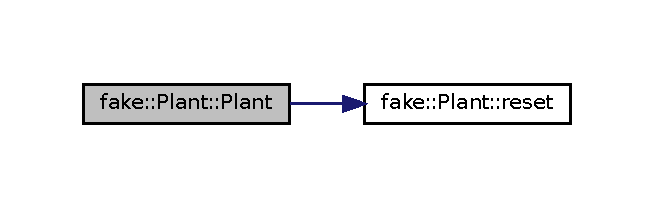
\includegraphics[width=314pt]{classfake_1_1_plant_a346cd2379207256138a0996960461d16_cgraph}
\end{center}
\end{figure}


\doxysubsection{Member Function Documentation}
\mbox{\Hypertarget{classfake_1_1_plant_a51e4596f215bec72d55bc4b4a568b8b0}\label{classfake_1_1_plant_a51e4596f215bec72d55bc4b4a568b8b0}} 
\index{fake::Plant@{fake::Plant}!command@{command}}
\index{command@{command}!fake::Plant@{fake::Plant}}
\doxysubsubsection{\texorpdfstring{command()}{command()}}
{\footnotesize\ttfamily void fake\+::\+Plant\+::command (\begin{DoxyParamCaption}\item[{const double}]{throttle,  }\item[{const double}]{steering,  }\item[{const double}]{dt }\end{DoxyParamCaption})}



Simulate an actual command to the vehicle. 

This is a very simple approximation of the plant; the throttle command is assumed to translate instantly into the new speed, and the new heading is calculated by integrating the effect of the new steering angle over the timestep.


\begin{DoxyParams}{Parameters}
{\em throttle} & The throttle command to apply. \\
\hline
{\em steering} & The steering command to apply. \\
\hline
{\em dt} & The time duration of the command. \\
\hline
\end{DoxyParams}
\mbox{\Hypertarget{classfake_1_1_plant_a65ac487259b9dc0e30f6495f5f5c0453}\label{classfake_1_1_plant_a65ac487259b9dc0e30f6495f5f5c0453}} 
\index{fake::Plant@{fake::Plant}!getState@{getState}}
\index{getState@{getState}!fake::Plant@{fake::Plant}}
\doxysubsubsection{\texorpdfstring{getState()}{getState()}}
{\footnotesize\ttfamily void fake\+::\+Plant\+::get\+State (\begin{DoxyParamCaption}\item[{double \&}]{speed,  }\item[{double \&}]{heading }\end{DoxyParamCaption}) const}



Get the current system state. 


\begin{DoxyParams}{Parameters}
{\em speed} & The current system speed. \\
\hline
{\em heading} & The current system heading. \\
\hline
\end{DoxyParams}
\mbox{\Hypertarget{classfake_1_1_plant_aa6f602aaabebcc84a03c2ae7a4878c05}\label{classfake_1_1_plant_aa6f602aaabebcc84a03c2ae7a4878c05}} 
\index{fake::Plant@{fake::Plant}!setState@{setState}}
\index{setState@{setState}!fake::Plant@{fake::Plant}}
\doxysubsubsection{\texorpdfstring{setState()}{setState()}}
{\footnotesize\ttfamily void fake\+::\+Plant\+::set\+State (\begin{DoxyParamCaption}\item[{const double}]{speed,  }\item[{const double}]{heading }\end{DoxyParamCaption})}



Set the current system state. 


\begin{DoxyParams}{Parameters}
{\em speed} & The new system speed. \\
\hline
{\em heading} & The new system heading. \\
\hline
\end{DoxyParams}


The documentation for this class was generated from the following files\+:\begin{DoxyCompactItemize}
\item 
include/fake/\mbox{\hyperlink{plant_8h}{plant.\+h}}\item 
app/fake/plant.\+cpp\end{DoxyCompactItemize}

\hypertarget{structfake_1_1_plant_options}{}\doxysection{fake\+::Plant\+Options Struct Reference}
\label{structfake_1_1_plant_options}\index{fake::PlantOptions@{fake::PlantOptions}}


Configurable parameters for the \mbox{\hyperlink{classfake_1_1_plant}{Plant}} class.  




{\ttfamily \#include $<$plant.\+h$>$}

\doxysubsection*{Public Member Functions}
\begin{DoxyCompactItemize}
\item 
\mbox{\hyperlink{structfake_1_1_plant_options_ad3757f5f0e5624335772a3d4c42ab91c}{Plant\+Options}} (double wheel\+\_\+base\+\_\+, double max\+\_\+steering\+\_\+angle\+\_\+)
\begin{DoxyCompactList}\small\item\em Constructor for \mbox{\hyperlink{structfake_1_1_plant_options}{Plant\+Options}} structure. \end{DoxyCompactList}\item 
\mbox{\Hypertarget{structfake_1_1_plant_options_a0326322942b8dd32a65a898a2403a1fe}\label{structfake_1_1_plant_options_a0326322942b8dd32a65a898a2403a1fe}} 
void \mbox{\hyperlink{structfake_1_1_plant_options_a0326322942b8dd32a65a898a2403a1fe}{print}} ()
\begin{DoxyCompactList}\small\item\em Print out the current set of state variables. \end{DoxyCompactList}\end{DoxyCompactItemize}
\doxysubsection*{Public Attributes}
\begin{DoxyCompactItemize}
\item 
\mbox{\Hypertarget{structfake_1_1_plant_options_ab136248a415d91829342f3f7249c3d90}\label{structfake_1_1_plant_options_ab136248a415d91829342f3f7249c3d90}} 
double \mbox{\hyperlink{structfake_1_1_plant_options_ab136248a415d91829342f3f7249c3d90}{wheel\+\_\+base}}
\begin{DoxyCompactList}\small\item\em Length between front and rear axles (m) \end{DoxyCompactList}\item 
\mbox{\Hypertarget{structfake_1_1_plant_options_a9161f2e40ab9030eeb46ad4ea297700e}\label{structfake_1_1_plant_options_a9161f2e40ab9030eeb46ad4ea297700e}} 
double \mbox{\hyperlink{structfake_1_1_plant_options_a9161f2e40ab9030eeb46ad4ea297700e}{max\+\_\+steering\+\_\+angle}}
\begin{DoxyCompactList}\small\item\em Maximum steering angle (rad) \end{DoxyCompactList}\item 
\mbox{\Hypertarget{structfake_1_1_plant_options_a3c98272e9031a261e4d3460a8bde633a}\label{structfake_1_1_plant_options_a3c98272e9031a261e4d3460a8bde633a}} 
double \mbox{\hyperlink{structfake_1_1_plant_options_a3c98272e9031a261e4d3460a8bde633a}{noise\+\_\+mean}} \{0.\+0\}
\begin{DoxyCompactList}\small\item\em Mean noise parameter for noise modeling. \end{DoxyCompactList}\item 
\mbox{\Hypertarget{structfake_1_1_plant_options_a381db64a553b56841feba39d723ecbf9}\label{structfake_1_1_plant_options_a381db64a553b56841feba39d723ecbf9}} 
double \mbox{\hyperlink{structfake_1_1_plant_options_a381db64a553b56841feba39d723ecbf9}{noise\+\_\+stddev}} \{0.\+0\}
\begin{DoxyCompactList}\small\item\em Std\+Dev noise parameter for noise modeling. \end{DoxyCompactList}\end{DoxyCompactItemize}


\doxysubsection{Detailed Description}
Configurable parameters for the \mbox{\hyperlink{classfake_1_1_plant}{Plant}} class. 

\doxysubsection{Constructor \& Destructor Documentation}
\mbox{\Hypertarget{structfake_1_1_plant_options_ad3757f5f0e5624335772a3d4c42ab91c}\label{structfake_1_1_plant_options_ad3757f5f0e5624335772a3d4c42ab91c}} 
\index{fake::PlantOptions@{fake::PlantOptions}!PlantOptions@{PlantOptions}}
\index{PlantOptions@{PlantOptions}!fake::PlantOptions@{fake::PlantOptions}}
\doxysubsubsection{\texorpdfstring{PlantOptions()}{PlantOptions()}}
{\footnotesize\ttfamily fake\+::\+Plant\+Options\+::\+Plant\+Options (\begin{DoxyParamCaption}\item[{double}]{wheel\+\_\+base\+\_\+,  }\item[{double}]{max\+\_\+steering\+\_\+angle\+\_\+ }\end{DoxyParamCaption})\hspace{0.3cm}{\ttfamily [inline]}}



Constructor for \mbox{\hyperlink{structfake_1_1_plant_options}{Plant\+Options}} structure. 


\begin{DoxyParams}{Parameters}
{\em wheel\+\_\+base} & Distance between front and rear axles (m) \\
\hline
{\em max\+\_\+steering\+\_\+angle} & Maximum steering angle (rad) \\
\hline
\end{DoxyParams}


The documentation for this struct was generated from the following file\+:\begin{DoxyCompactItemize}
\item 
include/fake/\mbox{\hyperlink{plant_8h}{plant.\+h}}\end{DoxyCompactItemize}

\hypertarget{class_window}{}\doxysection{Window Class Reference}
\label{class_window}\index{Window@{Window}}


G\+UI implementation for user interface.  




{\ttfamily \#include $<$window.\+h$>$}



Inheritance diagram for Window\+:
\nopagebreak
\begin{figure}[H]
\begin{center}
\leavevmode
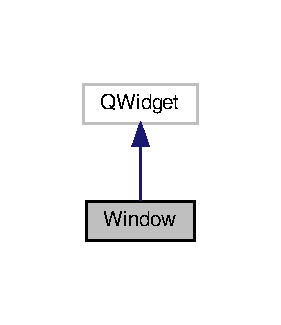
\includegraphics[width=139pt]{class_window__inherit__graph}
\end{center}
\end{figure}


Collaboration diagram for Window\+:
\nopagebreak
\begin{figure}[H]
\begin{center}
\leavevmode
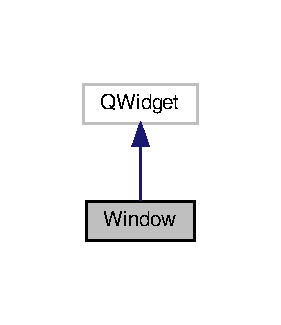
\includegraphics[width=139pt]{class_window__coll__graph}
\end{center}
\end{figure}
\doxysubsection*{Public Slots}
\begin{DoxyCompactItemize}
\item 
\mbox{\Hypertarget{class_window_afc02c9963511f615afb1c4ae92b53376}\label{class_window_afc02c9963511f615afb1c4ae92b53376}} 
void \mbox{\hyperlink{class_window_afc02c9963511f615afb1c4ae92b53376}{start}} ()
\begin{DoxyCompactList}\small\item\em Begin simulation run with current parameters. \end{DoxyCompactList}\item 
\mbox{\Hypertarget{class_window_a42353e5fb0b5670e6175709706670450}\label{class_window_a42353e5fb0b5670e6175709706670450}} 
void \mbox{\hyperlink{class_window_a42353e5fb0b5670e6175709706670450}{stop}} ()
\begin{DoxyCompactList}\small\item\em Stop current simulation run. \end{DoxyCompactList}\item 
\mbox{\Hypertarget{class_window_a00a00d153d98b446ec8b5b5ca870081d}\label{class_window_a00a00d153d98b446ec8b5b5ca870081d}} 
void \mbox{\hyperlink{class_window_a00a00d153d98b446ec8b5b5ca870081d}{reset}} ()
\begin{DoxyCompactList}\small\item\em Reset simulation to initial conditions. \end{DoxyCompactList}\end{DoxyCompactItemize}
\doxysubsection*{Public Member Functions}
\begin{DoxyCompactItemize}
\item 
\mbox{\Hypertarget{class_window_a8c86e48ef3180201cc97cb928abd66ca}\label{class_window_a8c86e48ef3180201cc97cb928abd66ca}} 
{\bfseries Window} (Q\+Widget $\ast$parent=nullptr)
\item 
\mbox{\hyperlink{class_window_adc0f6bc57df787f2ca22efb12ad2e6f9}{Window}} (const std\+::shared\+\_\+ptr$<$ \mbox{\hyperlink{structackermann_1_1_params}{ackermann\+::\+Params}} $>$ \&params, const std\+::shared\+\_\+ptr$<$ \mbox{\hyperlink{classackermann_1_1_controller}{ackermann\+::\+Controller}} $>$ \&controller, const std\+::shared\+\_\+ptr$<$ \mbox{\hyperlink{classfake_1_1_plant}{fake\+::\+Plant}} $>$ \&plant)
\begin{DoxyCompactList}\small\item\em Create G\+UI interface with pre-\/programmed conditions. \end{DoxyCompactList}\end{DoxyCompactItemize}


\doxysubsection{Detailed Description}
G\+UI implementation for user interface. 

\doxysubsection{Constructor \& Destructor Documentation}
\mbox{\Hypertarget{class_window_adc0f6bc57df787f2ca22efb12ad2e6f9}\label{class_window_adc0f6bc57df787f2ca22efb12ad2e6f9}} 
\index{Window@{Window}!Window@{Window}}
\index{Window@{Window}!Window@{Window}}
\doxysubsubsection{\texorpdfstring{Window()}{Window()}}
{\footnotesize\ttfamily Window\+::\+Window (\begin{DoxyParamCaption}\item[{const std\+::shared\+\_\+ptr$<$ \mbox{\hyperlink{structackermann_1_1_params}{ackermann\+::\+Params}} $>$ \&}]{params,  }\item[{const std\+::shared\+\_\+ptr$<$ \mbox{\hyperlink{classackermann_1_1_controller}{ackermann\+::\+Controller}} $>$ \&}]{controller,  }\item[{const std\+::shared\+\_\+ptr$<$ \mbox{\hyperlink{classfake_1_1_plant}{fake\+::\+Plant}} $>$ \&}]{plant }\end{DoxyParamCaption})}



Create G\+UI interface with pre-\/programmed conditions. 


\begin{DoxyParams}{Parameters}
{\em params} & Shared pointer to rover characteristic parameters \\
\hline
{\em controller} & Shared pointer to controller object \\
\hline
{\em plant} & Shared pointer to plant object (to simulate commands) \\
\hline
\end{DoxyParams}


The documentation for this class was generated from the following files\+:\begin{DoxyCompactItemize}
\item 
app/demo/\mbox{\hyperlink{window_8h}{window.\+h}}\item 
app/demo/\mbox{\hyperlink{window_8cpp}{window.\+cpp}}\end{DoxyCompactItemize}

\chapter{File Documentation}
\hypertarget{window_8cpp}{}\section{app/demo/window.cpp File Reference}
\label{window_8cpp}\index{app/demo/window.\+cpp@{app/demo/window.\+cpp}}
{\ttfamily \#include \char`\"{}demo/window.\+h\char`\"{}}\newline
{\ttfamily \#include $<$math.\+h$>$}\newline
{\ttfamily \#include $<$Q\+Check\+Box$>$}\newline
{\ttfamily \#include $<$Q\+Grid\+Layout$>$}\newline
{\ttfamily \#include $<$Q\+Group\+Box$>$}\newline
{\ttfamily \#include $<$Q\+Menu$>$}\newline
{\ttfamily \#include $<$Q\+Push\+Button$>$}\newline
{\ttfamily \#include $<$Q\+Radio\+Button$>$}\newline
{\ttfamily \#include $<$Q\+Double\+Spin\+Box$>$}\newline
Include dependency graph for window.\+cpp\+:
\nopagebreak
\begin{figure}[H]
\begin{center}
\leavevmode
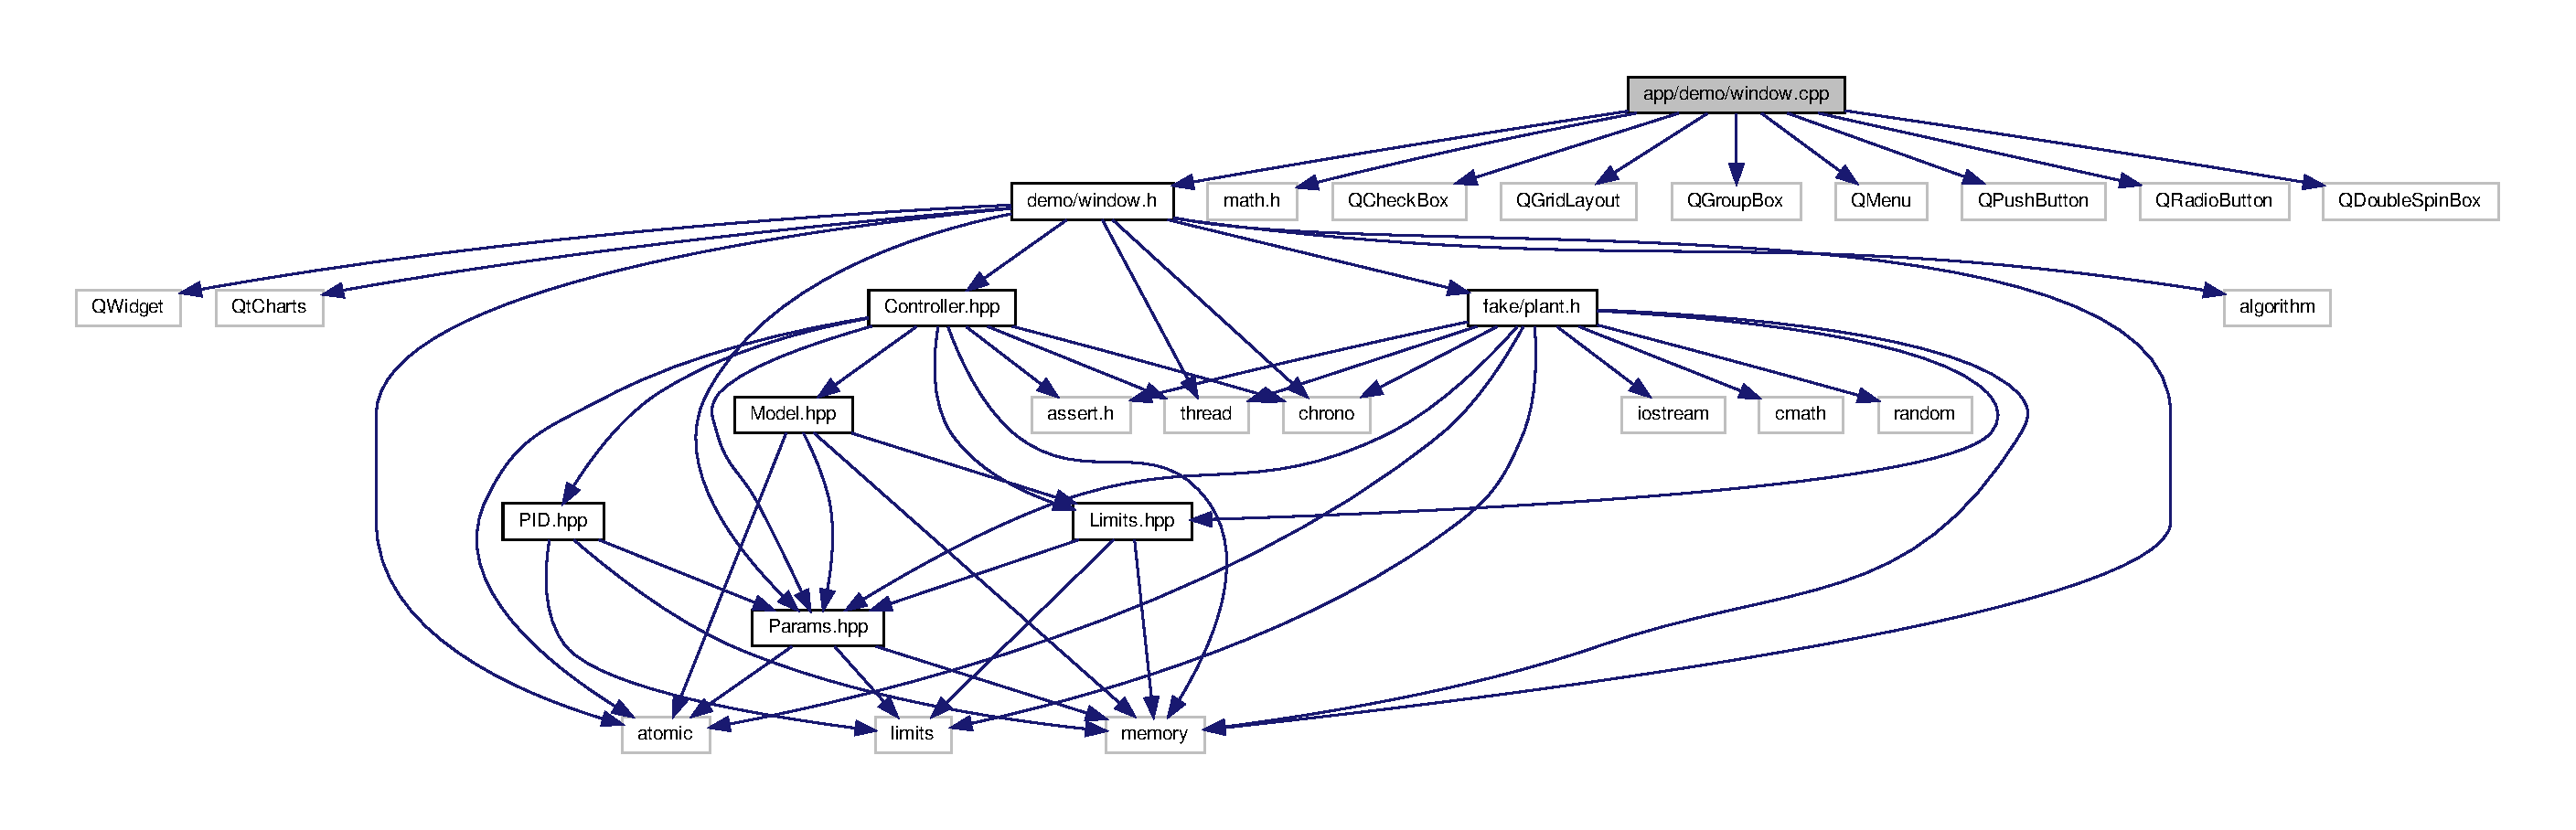
\includegraphics[width=350pt]{window_8cpp__incl}
\end{center}
\end{figure}


\subsection{Detailed Description}
\begin{DoxyCopyright}{Copyright}
Copyright \mbox{[}2020\mbox{]} Elyard/\+Kesani/\+Sahu 
\end{DoxyCopyright}

\hypertarget{window_8h}{}\section{app/demo/window.h File Reference}
\label{window_8h}\index{app/demo/window.\+h@{app/demo/window.\+h}}


Declaration for G\+UI implementation.  


{\ttfamily \#include $<$Q\+Widget$>$}\newline
{\ttfamily \#include $<$Qt\+Charts$>$}\newline
{\ttfamily \#include $<$fake/plant.\+h$>$}\newline
{\ttfamily \#include $<$memory$>$}\newline
{\ttfamily \#include $<$atomic$>$}\newline
{\ttfamily \#include $<$thread$>$}\newline
{\ttfamily \#include $<$chrono$>$}\newline
{\ttfamily \#include $<$algorithm$>$}\newline
{\ttfamily \#include $<$Params.\+hpp$>$}\newline
{\ttfamily \#include $<$Controller.\+hpp$>$}\newline
Include dependency graph for window.\+h\+:
\nopagebreak
\begin{figure}[H]
\begin{center}
\leavevmode
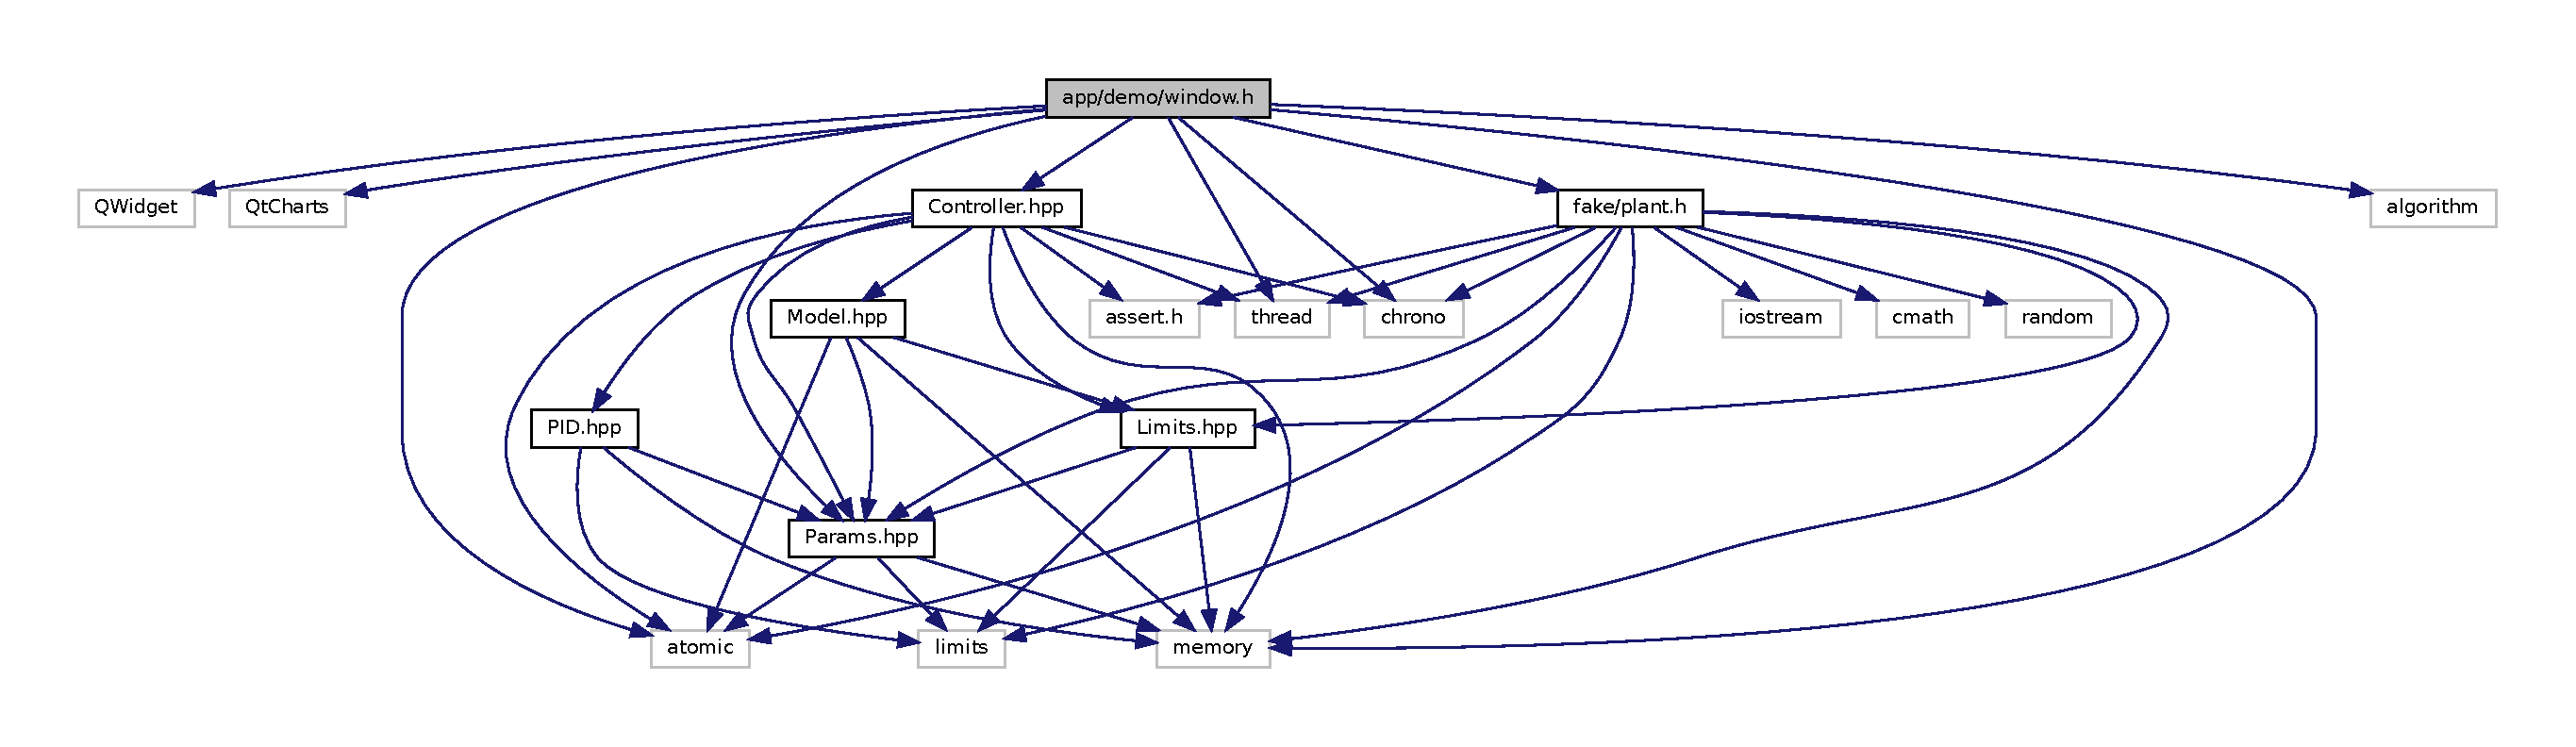
\includegraphics[width=350pt]{window_8h__incl}
\end{center}
\end{figure}
This graph shows which files directly or indirectly include this file\+:
\nopagebreak
\begin{figure}[H]
\begin{center}
\leavevmode
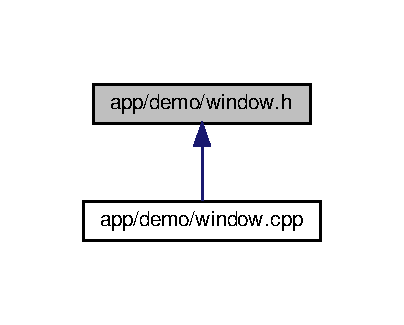
\includegraphics[width=194pt]{window_8h__dep__incl}
\end{center}
\end{figure}
\subsection*{Classes}
\begin{DoxyCompactItemize}
\item 
class \hyperlink{class_window}{Window}
\begin{DoxyCompactList}\small\item\em G\+UI implementation for user interface. \end{DoxyCompactList}\end{DoxyCompactItemize}
\subsection*{Macros}
\begin{DoxyCompactItemize}
\item 
\mbox{\Hypertarget{window_8h_a68ee019dafc12ee47d427cda7f17713e}\label{window_8h_a68ee019dafc12ee47d427cda7f17713e}} 
\#define {\bfseries T\+I\+M\+E\+S\+T\+EP}~0.\+1
\item 
\mbox{\Hypertarget{window_8h_a2e497a0b205edbcca17ef84ed4b7164c}\label{window_8h_a2e497a0b205edbcca17ef84ed4b7164c}} 
\#define {\bfseries T\+I\+M\+E\+W\+I\+N\+D\+OW}~10.\+0
\end{DoxyCompactItemize}


\subsection{Detailed Description}
Declaration for G\+UI implementation. 

\begin{DoxyAuthor}{Author}
Spencer Elyard 

Daniel M. Sahu 

Sentosh Kesani
\end{DoxyAuthor}
\begin{DoxyCopyright}{Copyright}
Copyright \mbox{[}2020\mbox{]} Elyard/\+Kesani/\+Sahu 
\end{DoxyCopyright}

\hypertarget{_limits_8cpp}{}\section{app/\+Limits.cpp File Reference}
\label{_limits_8cpp}\index{app/\+Limits.\+cpp@{app/\+Limits.\+cpp}}
{\ttfamily \#include $<$Limits.\+hpp$>$}\newline
{\ttfamily \#include $<$cmath$>$}\newline
Include dependency graph for Limits.\+cpp\+:
\nopagebreak
\begin{figure}[H]
\begin{center}
\leavevmode
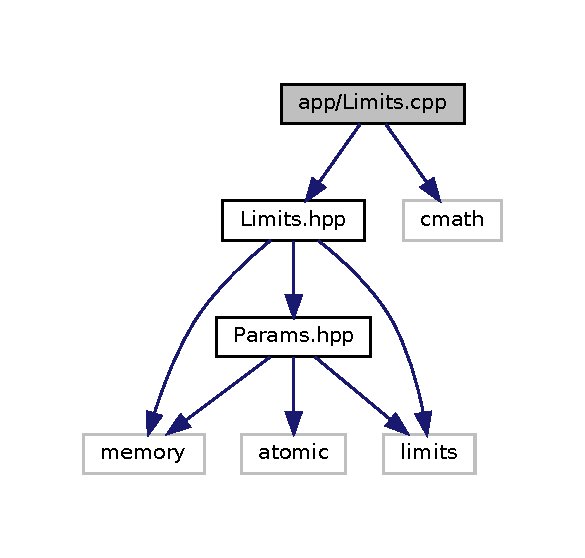
\includegraphics[width=264pt]{_limits_8cpp__incl}
\end{center}
\end{figure}
\subsection*{Namespaces}
\begin{DoxyCompactItemize}
\item 
 \hyperlink{namespaceackermann}{ackermann}
\begin{DoxyCompactList}\small\item\em Namespace for Ackermann controller implementation. \end{DoxyCompactList}\end{DoxyCompactItemize}


\subsection{Detailed Description}
\begin{DoxyAuthor}{Author}
Spencer Elyard 

Daniel M. Sahu 

Santosh Kesani
\end{DoxyAuthor}
\begin{DoxyCopyright}{Copyright}
\mbox{[}2020\mbox{]} 
\end{DoxyCopyright}

\hypertarget{_controller_8hpp}{}\doxysection{include/\+Controller.hpp File Reference}
\label{_controller_8hpp}\index{include/Controller.hpp@{include/Controller.hpp}}


Class declaration for top level A\+C\+ME Ackermann Controller.  


{\ttfamily \#include $<$assert.\+h$>$}\newline
{\ttfamily \#include $<$atomic$>$}\newline
{\ttfamily \#include $<$memory$>$}\newline
{\ttfamily \#include $<$thread$>$}\newline
{\ttfamily \#include $<$chrono$>$}\newline
{\ttfamily \#include \char`\"{}Params.\+hpp\char`\"{}}\newline
{\ttfamily \#include \char`\"{}Model.\+hpp\char`\"{}}\newline
{\ttfamily \#include \char`\"{}P\+I\+D.\+hpp\char`\"{}}\newline
{\ttfamily \#include \char`\"{}Limits.\+hpp\char`\"{}}\newline
Include dependency graph for Controller.\+hpp\+:
\nopagebreak
\begin{figure}[H]
\begin{center}
\leavevmode
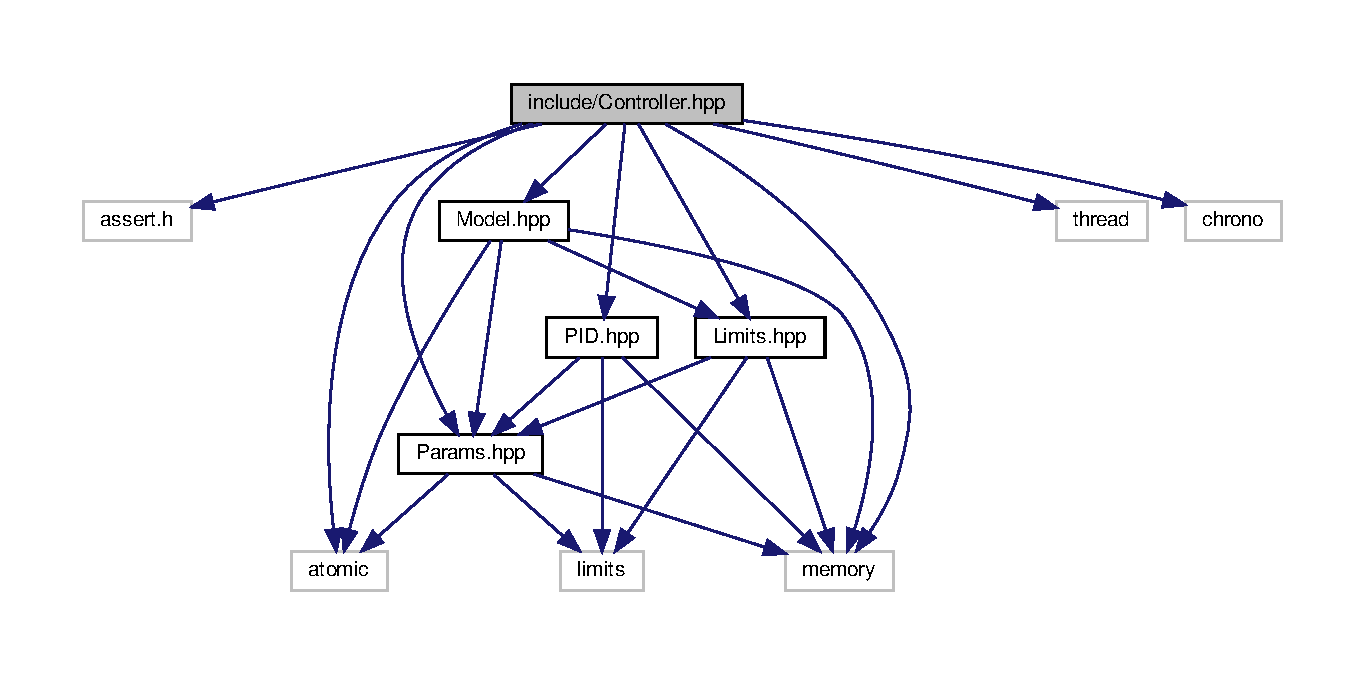
\includegraphics[width=350pt]{_controller_8hpp__incl}
\end{center}
\end{figure}
This graph shows which files directly or indirectly include this file\+:
\nopagebreak
\begin{figure}[H]
\begin{center}
\leavevmode
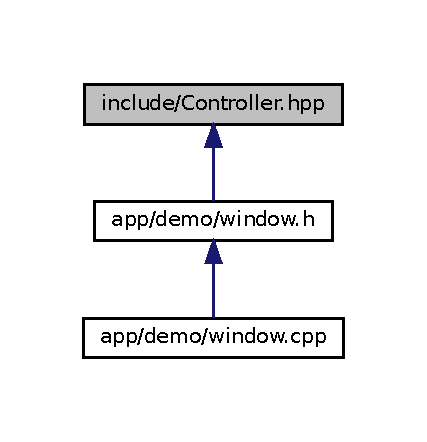
\includegraphics[width=205pt]{_controller_8hpp__dep__incl}
\end{center}
\end{figure}
\doxysubsection*{Classes}
\begin{DoxyCompactItemize}
\item 
class \mbox{\hyperlink{classackermann_1_1_controller}{ackermann\+::\+Controller}}
\begin{DoxyCompactList}\small\item\em Implementation of a steering and speed controller for a rover with an Ackermann steering mechanism. \end{DoxyCompactList}\end{DoxyCompactItemize}
\doxysubsection*{Namespaces}
\begin{DoxyCompactItemize}
\item 
 \mbox{\hyperlink{namespaceackermann}{ackermann}}
\begin{DoxyCompactList}\small\item\em Namespace for Ackermann controller implementation. \end{DoxyCompactList}\end{DoxyCompactItemize}


\doxysubsection{Detailed Description}
Class declaration for top level A\+C\+ME Ackermann Controller. 

\begin{DoxyAuthor}{Author}
Spencer Elyard 

Daniel M. Sahu 

Santosh Kesani 
\end{DoxyAuthor}
\begin{DoxyCopyright}{Copyright}
\mbox{[}2020\mbox{]} 
\end{DoxyCopyright}

\hypertarget{plant_8h}{}\doxysection{include/fake/plant.h File Reference}
\label{plant_8h}\index{include/fake/plant.h@{include/fake/plant.h}}


A Fake implementation of a physical Ackermann platform.  


{\ttfamily \#include $<$assert.\+h$>$}\newline
{\ttfamily \#include $<$iostream$>$}\newline
{\ttfamily \#include $<$limits$>$}\newline
{\ttfamily \#include $<$cmath$>$}\newline
{\ttfamily \#include $<$random$>$}\newline
{\ttfamily \#include $<$atomic$>$}\newline
{\ttfamily \#include $<$memory$>$}\newline
{\ttfamily \#include $<$thread$>$}\newline
{\ttfamily \#include $<$chrono$>$}\newline
{\ttfamily \#include \char`\"{}Params.\+hpp\char`\"{}}\newline
{\ttfamily \#include \char`\"{}Limits.\+hpp\char`\"{}}\newline
Include dependency graph for plant.\+h\+:\nopagebreak
\begin{figure}[H]
\begin{center}
\leavevmode
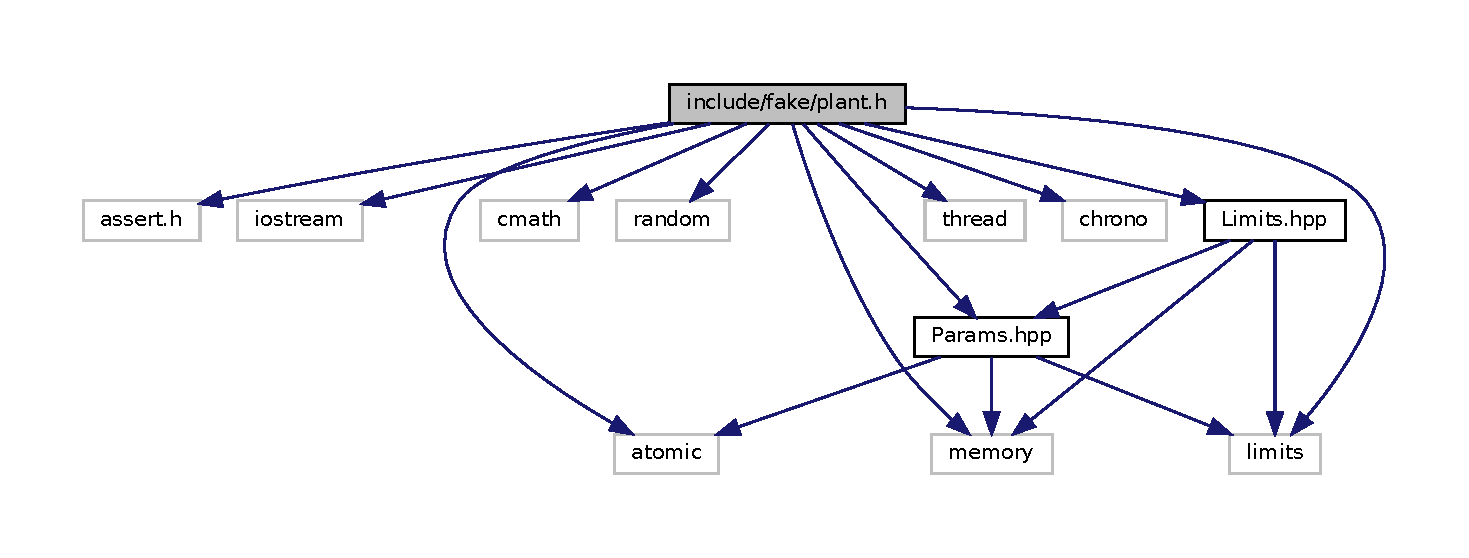
\includegraphics[width=350pt]{plant_8h__incl}
\end{center}
\end{figure}
This graph shows which files directly or indirectly include this file\+:\nopagebreak
\begin{figure}[H]
\begin{center}
\leavevmode
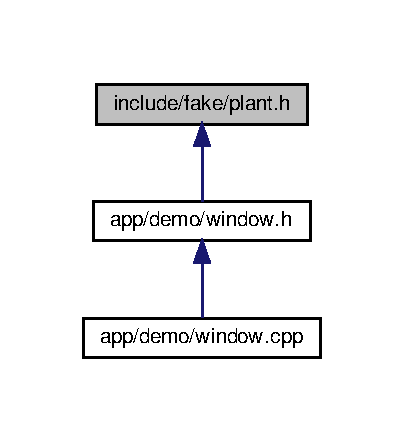
\includegraphics[width=194pt]{plant_8h__dep__incl}
\end{center}
\end{figure}
\doxysubsection*{Classes}
\begin{DoxyCompactItemize}
\item 
struct \mbox{\hyperlink{structfake_1_1_plant_options}{fake\+::\+Plant\+Options}}
\begin{DoxyCompactList}\small\item\em Configurable parameters for the \mbox{\hyperlink{classfake_1_1_plant}{Plant}} class. \end{DoxyCompactList}\item 
class \mbox{\hyperlink{classfake_1_1_plant}{fake\+::\+Plant}}
\begin{DoxyCompactList}\small\item\em A Fake \mbox{\hyperlink{classfake_1_1_plant}{Plant}} for use in testing our Controller. \end{DoxyCompactList}\end{DoxyCompactItemize}
\doxysubsection*{Namespaces}
\begin{DoxyCompactItemize}
\item 
 \mbox{\hyperlink{namespacefake}{fake}}
\begin{DoxyCompactList}\small\item\em Namespace for fake plant model implementation. \end{DoxyCompactList}\end{DoxyCompactItemize}


\doxysubsection{Detailed Description}
A Fake implementation of a physical Ackermann platform. 

\begin{DoxyAuthor}{Author}
Daniel M.
\end{DoxyAuthor}
\begin{DoxyCopyright}{Copyright}
\mbox{[}2020\mbox{]} 
\end{DoxyCopyright}

\hypertarget{_limits_8hpp}{}\doxysection{include/\+Limits.hpp File Reference}
\label{_limits_8hpp}\index{include/Limits.hpp@{include/Limits.hpp}}


Class declaration for Limits class.  


{\ttfamily \#include $<$memory$>$}\newline
{\ttfamily \#include $<$limits$>$}\newline
{\ttfamily \#include \char`\"{}Params.\+hpp\char`\"{}}\newline
Include dependency graph for Limits.\+hpp\+:\nopagebreak
\begin{figure}[H]
\begin{center}
\leavevmode
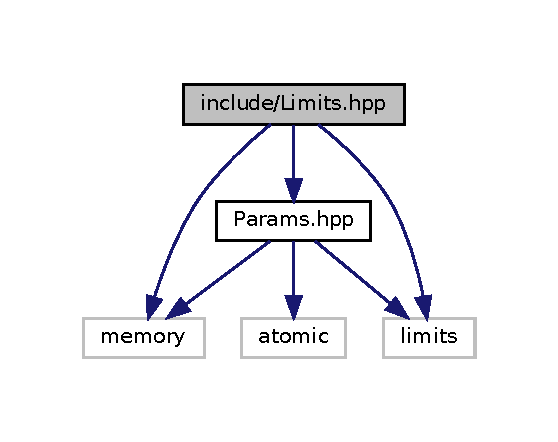
\includegraphics[width=268pt]{_limits_8hpp__incl}
\end{center}
\end{figure}
This graph shows which files directly or indirectly include this file\+:\nopagebreak
\begin{figure}[H]
\begin{center}
\leavevmode
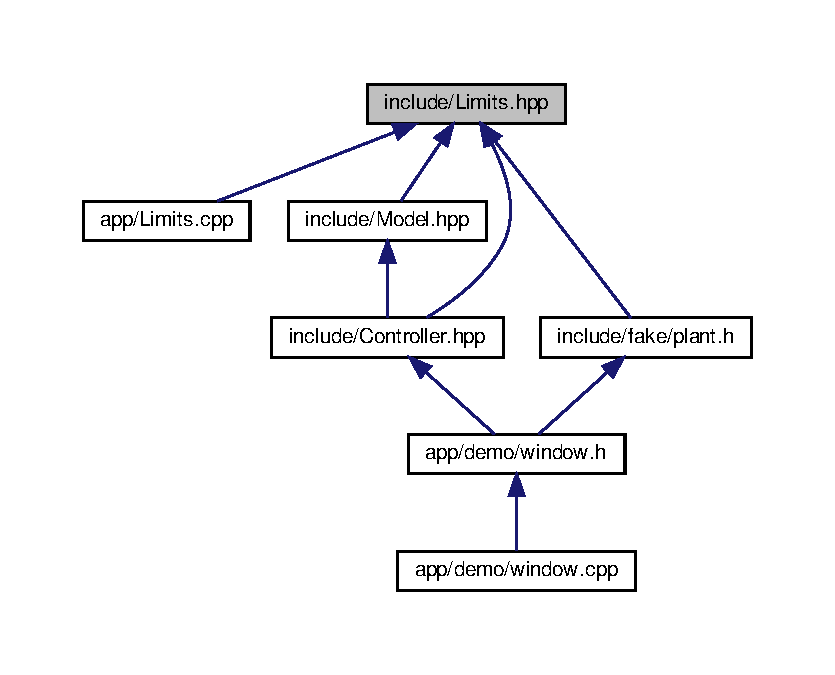
\includegraphics[width=336pt]{_limits_8hpp__dep__incl}
\end{center}
\end{figure}
\doxysubsection*{Classes}
\begin{DoxyCompactItemize}
\item 
class \mbox{\hyperlink{classackermann_1_1_limits}{ackermann\+::\+Limits}}
\begin{DoxyCompactList}\small\item\em Class used to apply known limits to a given desired control signal. \end{DoxyCompactList}\end{DoxyCompactItemize}
\doxysubsection*{Namespaces}
\begin{DoxyCompactItemize}
\item 
 \mbox{\hyperlink{namespaceackermann}{ackermann}}
\begin{DoxyCompactList}\small\item\em Namespace for Ackermann controller implementation. \end{DoxyCompactList}\end{DoxyCompactItemize}


\doxysubsection{Detailed Description}
Class declaration for Limits class. 

Object containing limitations for the Ackermann rover to prevent sending steering or speed commands past allowable bounds.

\begin{DoxyAuthor}{Author}
Spencer Elyard 

Daniel M. Sahu 

Santosh Kesani 
\end{DoxyAuthor}
\begin{DoxyCopyright}{Copyright}
\mbox{[}2020\mbox{]} 
\end{DoxyCopyright}

\hypertarget{_model_8hpp}{}\section{include/\+Model.hpp File Reference}
\label{_model_8hpp}\index{include/\+Model.\+hpp@{include/\+Model.\+hpp}}


Class declaration for an Ackermann vehicle model.  


{\ttfamily \#include $<$memory$>$}\newline
{\ttfamily \#include $<$atomic$>$}\newline
{\ttfamily \#include \char`\"{}Params.\+hpp\char`\"{}}\newline
{\ttfamily \#include \char`\"{}Limits.\+hpp\char`\"{}}\newline
Include dependency graph for Model.\+hpp\+:
\nopagebreak
\begin{figure}[H]
\begin{center}
\leavevmode
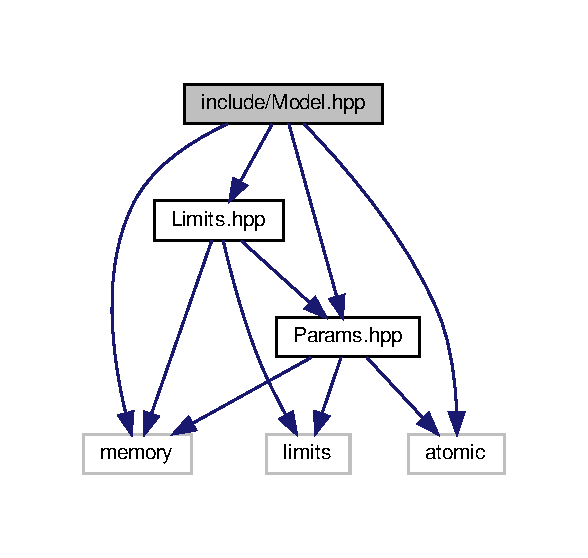
\includegraphics[width=282pt]{_model_8hpp__incl}
\end{center}
\end{figure}
This graph shows which files directly or indirectly include this file\+:
\nopagebreak
\begin{figure}[H]
\begin{center}
\leavevmode
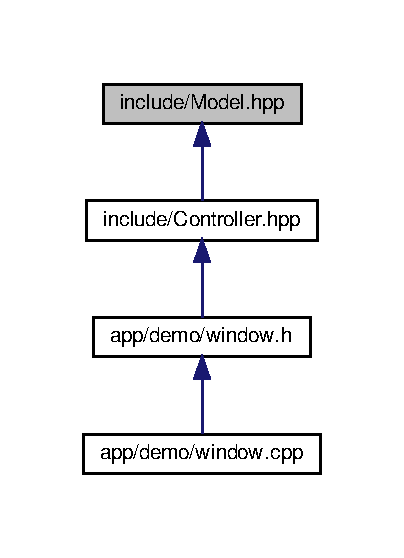
\includegraphics[width=194pt]{_model_8hpp__dep__incl}
\end{center}
\end{figure}
\subsection*{Classes}
\begin{DoxyCompactItemize}
\item 
class \hyperlink{classackermann_1_1_model}{ackermann\+::\+Model}
\begin{DoxyCompactList}\small\item\em This class is used to further define a vehicle with Ackermann steering. \end{DoxyCompactList}\end{DoxyCompactItemize}
\subsection*{Namespaces}
\begin{DoxyCompactItemize}
\item 
 \hyperlink{namespaceackermann}{ackermann}
\begin{DoxyCompactList}\small\item\em Namespace for Ackermann controller implementation. \end{DoxyCompactList}\end{DoxyCompactItemize}


\subsection{Detailed Description}
Class declaration for an Ackermann vehicle model. 

\begin{DoxyAuthor}{Author}
Spencer Elyard 

Daniel M. Sahu 
\end{DoxyAuthor}
\begin{DoxyCopyright}{Copyright}
\mbox{[}2020\mbox{]} 
\end{DoxyCopyright}

\hypertarget{_params_8hpp}{}\doxysection{include/\+Params.hpp File Reference}
\label{_params_8hpp}\index{include/Params.hpp@{include/Params.hpp}}


Parameters used in the Ackermann controller system.  


{\ttfamily \#include $<$memory$>$}\newline
{\ttfamily \#include $<$atomic$>$}\newline
{\ttfamily \#include $<$limits$>$}\newline
Include dependency graph for Params.\+hpp\+:\nopagebreak
\begin{figure}[H]
\begin{center}
\leavevmode
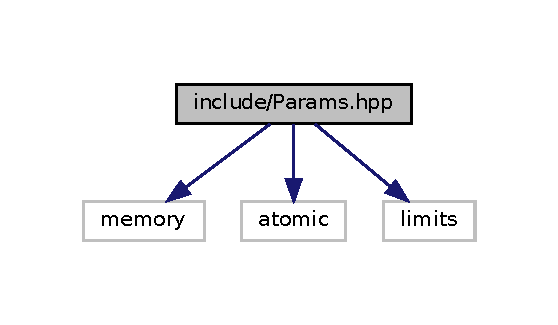
\includegraphics[width=268pt]{_params_8hpp__incl}
\end{center}
\end{figure}
This graph shows which files directly or indirectly include this file\+:\nopagebreak
\begin{figure}[H]
\begin{center}
\leavevmode
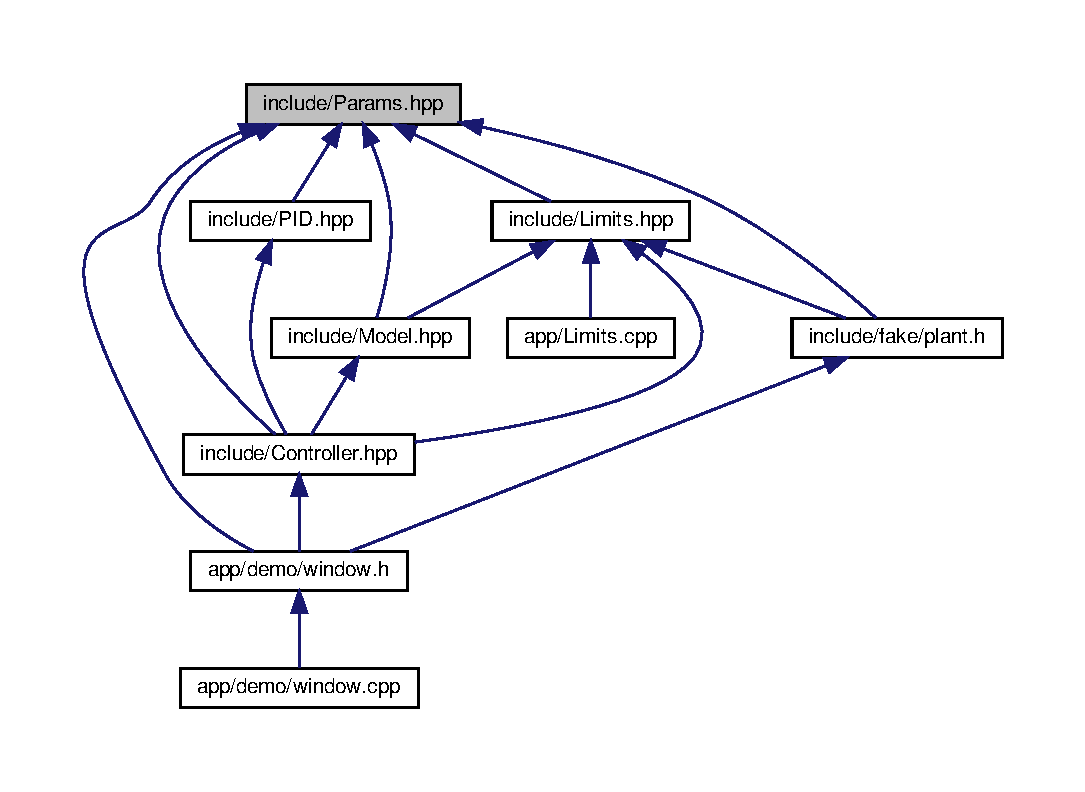
\includegraphics[width=350pt]{_params_8hpp__dep__incl}
\end{center}
\end{figure}
\doxysubsection*{Classes}
\begin{DoxyCompactItemize}
\item 
struct \mbox{\hyperlink{structackermann_1_1_p_i_d_params}{ackermann\+::\+P\+I\+D\+Params}}
\begin{DoxyCompactList}\small\item\em Structure containing \mbox{\hyperlink{classackermann_1_1_p_i_d}{P\+ID}} parameters. \end{DoxyCompactList}\item 
struct \mbox{\hyperlink{structackermann_1_1_params}{ackermann\+::\+Params}}
\begin{DoxyCompactList}\small\item\em Structure containing rover characteristics and limitations. \end{DoxyCompactList}\end{DoxyCompactItemize}
\doxysubsection*{Namespaces}
\begin{DoxyCompactItemize}
\item 
 \mbox{\hyperlink{namespaceackermann}{ackermann}}
\begin{DoxyCompactList}\small\item\em Namespace for Ackermann controller implementation. \end{DoxyCompactList}\end{DoxyCompactItemize}


\doxysubsection{Detailed Description}
Parameters used in the Ackermann controller system. 

\begin{DoxyAuthor}{Author}
Spencer Elyard 

Daniel M. Sahu 

Santosh Kesani 
\end{DoxyAuthor}
\begin{DoxyCopyright}{Copyright}
\mbox{[}2020\mbox{]} 
\end{DoxyCopyright}

\hypertarget{_p_i_d_8hpp}{}\doxysection{include/\+P\+ID.hpp File Reference}
\label{_p_i_d_8hpp}\index{include/PID.hpp@{include/PID.hpp}}


Class declaration for a P\+ID controller.  


{\ttfamily \#include $<$memory$>$}\newline
{\ttfamily \#include $<$limits$>$}\newline
{\ttfamily \#include $<$Params.\+hpp$>$}\newline
Include dependency graph for P\+I\+D.\+hpp\+:\nopagebreak
\begin{figure}[H]
\begin{center}
\leavevmode
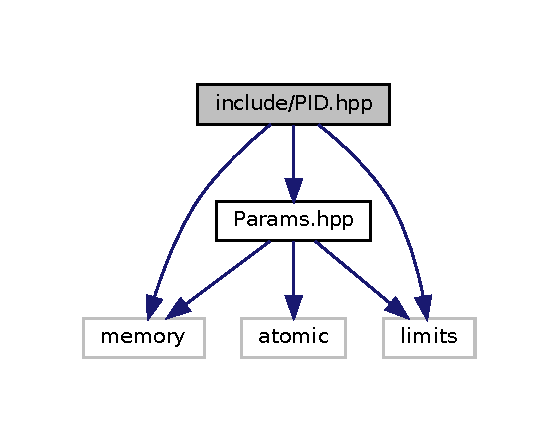
\includegraphics[width=268pt]{_p_i_d_8hpp__incl}
\end{center}
\end{figure}
This graph shows which files directly or indirectly include this file\+:\nopagebreak
\begin{figure}[H]
\begin{center}
\leavevmode
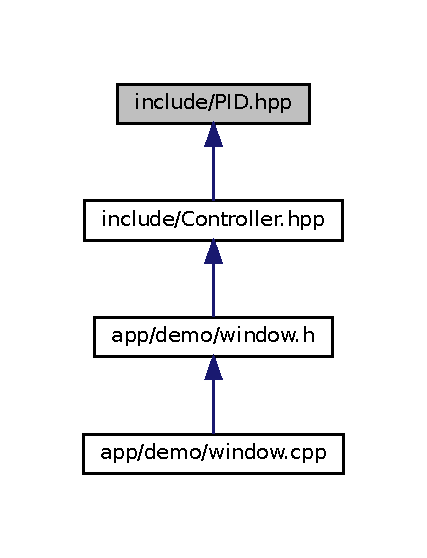
\includegraphics[width=204pt]{_p_i_d_8hpp__dep__incl}
\end{center}
\end{figure}
\doxysubsection*{Classes}
\begin{DoxyCompactItemize}
\item 
class \mbox{\hyperlink{classackermann_1_1_p_i_d}{ackermann\+::\+P\+ID}}
\begin{DoxyCompactList}\small\item\em This class implements a \mbox{\hyperlink{classackermann_1_1_p_i_d}{P\+ID}} controller with max/min clamping of output values to prevent integral windup. \end{DoxyCompactList}\end{DoxyCompactItemize}
\doxysubsection*{Namespaces}
\begin{DoxyCompactItemize}
\item 
 \mbox{\hyperlink{namespaceackermann}{ackermann}}
\begin{DoxyCompactList}\small\item\em Namespace for Ackermann controller implementation. \end{DoxyCompactList}\end{DoxyCompactItemize}


\doxysubsection{Detailed Description}
Class declaration for a P\+ID controller. 

\begin{DoxyAuthor}{Author}
Spencer Elyard 

Daniel M. Sahu 

Santosh Kesani 
\end{DoxyAuthor}
\begin{DoxyCopyright}{Copyright}
\mbox{[}2020\mbox{]} 
\end{DoxyCopyright}

%--- End generated contents ---

% Index
\backmatter
\newpage
\phantomsection
\clearemptydoublepage
\addcontentsline{toc}{chapter}{Index}
\printindex

\end{document}
